\documentclass[defaultstyle,11pt]{thesis}

\usepackage{amssymb}		% to get all AMS symbols
\usepackage[colorlinks=true, allcolors=blue]{hyperref}
\usepackage{subcaption}
\usepackage{dirtree}
\usepackage{xcolor}
\usepackage{amsmath}
\usepackage{graphicx}
\usepackage[utf8]{inputenc}
\usepackage{amsfonts}
\usepackage{algorithm}
\usepackage{algpseudocode}


%%%%%%%%%%%%   All the preamble material:   %%%%%%%%%%%%

\title{Solar Active Region Parameterization and Segmentation}

\author{T.~J.}{Lincke}

\otherdegrees{}

\degree{Bachelors of Science, Computer Science}		%  #1 {long descr.}
	{BS Computer Science}		%  #2 {short descr.}

\dept{Department of}			%  #1 {designation}
	{Computer Science}		%  #2 {name}

\advisor{Prof.}				%  #1 {title}
	{Elizabeth Bradley}			%  #2 {name}

\reader{Thomas Berger}		%  2nd person to sign thesis
\readerThree{David Quigley}		%  3rd person to sign thesis

\abstract{  	% because it is very short
    This thesis study presents a novel feature extraction method for machine learning applications in solar flare forecasting (phrased in a classification problem space). The feature extraction algorithm computes 58 defined physical values from four chosen salient segments of an active solar region, a region on the sun's surface with high magnetic flux. These segments include the neutral line (a region of high magnetic flux gradient), umbra, and penumbra (distinctly structured regions visible to the naked eye). This study's precise problem space determines if an AR will produce a type M or X (or M+, referring to the two most intense types of flares) flare in the next 24 hours.
    
    I show that active region segmentation, followed by extracting physical features from the resultant segments, creates a more meaningful and informative feature-set for machine learning tasks than the same physical features extracted on the original active region. I will (1) compare various machine learning methods to show that many (in fact, all) of a set of machine learning models perform better on the Segmented feature set. Then I will (2) focus on only the top-performing model (an artificial neural network - ANN) and describe the benefits/drawbacks and how I can change the problem space and optimize the model to make it the most useful in practice. 
    
    I collected four feature sets on 145,916 AR images from 787 distinct active regions that did or did not produce an M+ class flare within 24 hours. By default, each of these images included the \textit{SHARPs} feature set, which is a set of physical features extracted by the Joint Scientific Operations Center (JSOC) on the entire active region. I will treat the SHARPs feature set as a control meant to represent the current status of flare forecasting feature sets in practice. Next was the \textit{Full} feature set, which is a new set consisting of 58 physical quantities extracted (and I compute the first four statistical moments) on the entire active region, creating a controlled standard for which the same features extracted on a segmented active region can compare in the \textit{Segmented} feature set. Contrasting the results of the Full and Segmented feature sets will help in the first goal mentioned in the previous paragraph. Comparing the results of the Segmented feature set and SHARPs feature set will help progress towards goal two. In the ANN the average True Skill Statistic score (TSS) for the Segmented feature set was $0.787 \pm 0.05$, the average TSS score for the feature set without segmentation (Full) was $0.759 \pm 0.04$, and the average TSS score for a feature set widely used in other research (SHARPs feature set) was $0.676 \pm 0.06$.
    
    The fourth feature set is called the \textit{Graph} feature set. The Graph feature set is an extension of the Segmented feature set, where instead of treating each salient sub-region as a single object, clusters of disjoint subregions are considered nodes in a Graph, with edges existing between segments that are near one another. However, my findings showed little initial success with this feature set for automated flare forecasting due to its extremely high complexity, parameter tuning, and computation expense. Although promising as an arbitrary extension of traditional human-centric flare classification methods such as the McIntosh system, in practice, there are too many free variables to tune and too much variance in active solar regions for this feature set to be used without a critical human eye to analyze each data point for edge and boundary conditions. Therefore, this thesis will show how the Graph feature set is a valuable tool for a trained solar physicist's eye but not as valuable for automated solar flare forecasting.
}

\IRBprotocol{E927F29.001X}	% optional!

\ToCisShort	% use this only for 1-page Table of Contents

\LoFisShort	% use this only for 1-page Table of Figures
% \emptyLoF	% use this if there is no List of Figures

\LoTisShort	% use this only for 1-page Table of Tables
% \emptyLoT	% use this if there is no List of Tables

%%%%%%%%%%%%%%%%%%%%%%%%%%%%%%%%%%%%%%%%%%%%%%%%%%%%%%%%%%%%%%%%%
%%%%%%%%%%%%%%%       BEGIN DOCUMENT...         %%%%%%%%%%%%%%%%%
%%%%%%%%%%%%%%%%%%%%%%%%%%%%%%%%%%%%%%%%%%%%%%%%%%%%%%%%%%%%%%%%%
\begin{document}

\input macros.tex

\chapter{Introduction}
\label{chp:introduction}

\section{Context}
The remarkably complex and dynamic nature of the photosphere (the layer of the sun's atmosphere visible to the eye) allows for the accumulation of magnetic field in clustered areas known as ``Active Regions" (ARs). Over time, as these regions grow, the magnetic field lines intertwine, forming magnetic flux ropes. These flux ropes are a collection of magnetic field lines and active plasma from the sun's surface that, if large enough, erupt to produce solar flares. When these eruptions are energetic, they release a large mass of plasma and magnetic field into interplanetary space known as a Coronal Mass Ejection (CME). Naturally, being able to predict when a solar eruption occurs is of utmost importance for the prediction of ``Space Weather" near earth. When CMEs impact the earth's magnetosphere, the ensuing geomagnetic storms cause a large current and magnetic field to propagate through the ionosphere, causing the upper atmosphere to expand, increasing drag on satellites, and causing currents to surge through long conductors on the ground like the power grid. The power grid picks these geomagnetically induced currents up, which can cause blackouts and damage to our electrical infrastructure. 

Some flare prediction in the past has involved classification based on physical properties such as $H_{\alpha}$ bands \cite{hale_magnetic_1919}, or the Ising number of the most active magnetic regions \cite{MCintosh}. Mathematical models such as the one described by Heyvaerts et al. \cite{heyvaerts_mathematical_1983} analyze the asymptotic behavior of solar flares as a series of partial differential equations, or the static solutions of magnetohydrodynamical systems of partial differential equations. Other visually-based forecasting methods exist, such as the McIntosh scale \cite{MCintosh}, which takes the visual characteristics of an AR and matches them to a look-up table of climatalogical flaring probability.

However, the above physical and visual feature-based forecasting methods fall short in that they are either highly simplified physical models or too sensitive to initial conditions and the seemingly chaotic surface of the sun makes it hard to propagate results through time. Physical models such as the CSHKP model \cite{choudhary_strassmeier_2011} of magnetic reconnection treat a flare as an idealized magnetic field that remains static in time. Mathematical models often assume a force-free magnetic field and quasi-static evolution, a harsh oversimplification.

A recent innovation in flare prediction is Topological Data Analysis (TDA) which analyzes the mathematical shape of an AR. The number of holes and components in an AR can be used as features in machine learning models and because of the flexibility of modern neural networks, it is possible to design an algorithm, find more features (topological, geometric, and physical in this case), then inject them as inputs without actually changing much of the underlying algorithm. TDA of ARs could yield insight into when ARs grow in complexity and how they evolve and the success of TDA hints that their unique sub-regions better describe ARs. A ``hole" in an AR is simply a more dense \textbf{connected} subset of the magnetic field. Therefore, rather than heuristically measuring topological properties, I have chosen to define what a connected subset actually is in an AR (an umbra/penumbra combination). Extracting this region and running similar tests as have been done before to the entire AR will result in better performance than simply extracting physical features from the entire AR. 

\section{Relevant Work}
\label{relevantworkchap}

Recently, flare forecasting methods have seen an uptick, with many reviews on the effectiveness and accuracy of each method (see \cite{Comparison1} \cite{Comparison2} \cite{Comparison3} \cite{Comparison4}). Deshmukh et al. \cite{varad} use Topological Data Analysis (TDA) to forecast flares and makes use of persistent homology diagrams to measure the number and prominence of topological ``1-holes" in an AR magnetogram. This method motivates my thesis because the segmentation of an AR into distinct subregions takes topological information (holes and subregions) and computes physical features for each isolated region. Deshmukh et al. extracts topological features (in the form of a persistence diagram) and passes this vector through a four-layer artificial neural network (ANN) constructed using PyTorch \cite{pytorch}. Compared to the same neural network with 19 different SHARP features (on the entire AR), the topological approach performed just as well as the physics-based featurization. The topological feature set alone resulted in a $0.90 \pm 0.01$ accuracy, and the SHARP parameterization resulted in a $0.89 \pm 0.01$ accuracy. Note that \textit{accuracy} is defined as the number of correct predictions (true positives plus true negatives) over the total number of attempted predictions. There are better scoring methods (see appendix \ref{appendix:judjingcriteria}) that take into account a large number of non-flaring regions within the feature set. \footnote{In fact, the Heidke skill score (the score I will use to address this problem) of Deshmukh et al. model using topology alone is $0.16 \pm 0.02$ where the SHARP features are lower at $0.13 \pm 0.01$}.

% TODO
This problem is inherently three-dimensional (as opposed to the data provided by the Solar Dynamics Observatory (SDO), which are images of the photospheric surface rather than the three-dimensional samples. Many methods attempt to describe the three-dimensional nature of AR to predict magnetic reconnection. Georgoulis et al. \cite{georgoulis_rust_2007} uses a method that measures the effective magnetic field ($B_{eff}$) in order to predict coronal connectivity as a metric for flaring.

On the other hand, removing the three-dimensional restriction based on a ``force-free" or zero net current models, it is hypothesized by Lekka et al. \cite{Properties1} that the parameterization of the solar surface using various physical metrics (total unsigned flux, total magnetic twist, etc.) is an efficient method for flare forecasting. Choudhary et al. \cite{choudhary_strassmeier_2011} and Yuan et al. \cite{yuan_shih_jing_wang_2010} use a method that computes total magnetic unsigned flux (one of the highest indications of flaring), length of the neutral line and total magnetic energy dissipation and uses this data with various machine learning methods. Similarly, Falconer et al. \cite{falconer_moore_gary_2008} measure the free magnetic energy inside strong gradient neutral lines and then use least squares to convert this distribution through Poisson statistics. This method works best for flares of class C1 or more. Using the same strong gradient neutral lines as a restricted domain, Schrijver \cite{schrijver} measures the magnetic field close to non-potential high gradient neutral lines in order to compute the $R$ parameter - the total adjacent flux to polarity inversion lines. In another primary motivation for this paper, Barnes et al. \cite{Properties1} measures many AR physical scalar quantities and performs a discriminant analysis to cluster flaring and non-flaring regions. The third paper of Barnes et al. \cite{Properties3} describes Magnetic Charge Topology (MCT) and partitions flux based on the primary charge sign. They use the current free potential to simulate coronal connections and magnetic reconnection.

Other non-physical features that measure more of the geometry of the AR have been used, such as the capacity or fractal dimension of the umbra and penumbra in Mcateer et al. \cite{mcateer_gallagher_conlon_2010}. This feature is motivated by flares that often occur in twisted and complicated-looking boundaries between highly positive and negative regions which is expressed using the capacity dimension. Higgins et al. \cite{higgins_gallagher_mcateer_bloomfield_2011} produced another geometric approach to parameterization, designing Solar Monitor AR Tracker (SMART) to measure the area and flux of ARs as well as spatial properties and length of the neutral line, SMART feeds these parameters through a machine learning algorithm as features. Visual geometric properties have been encoded in the classical McIntosh \cite{MCintosh} classification system. The McIntosh class of an AR, as well as how this class changes through time, has been used in Automated Solar Activity Prediction (ASAP) \cite{colak_qahwaji_2007} \cite{colak_qahwaji_2009}. Colak et al. use the McIntosh class as a parameter for logistic regression and support vector machines.

The methods above have been used alone and in ensemble to predict flares. However, the Space Weather Prediction Center (SWPC) uses a team of educated forecasters who examine ARs by eye and categorize them based on their McIntosh \cite{MCintosh} scale.  \cite{VerificationCurrentMethod} conducts a review of the efficiency of this method, but it is very subjective. It was shown in \cite{VerificationCurrentMethod} that forecaster experience affects their decision accuracy, which is typically only slightly above simply labeling all images as non-flaring, even for experienced forecasters.

\section{Problem Space}
\label{sec:problemspace}

NASA's Solar Dynamics Observatory satellite has collected magnetograms (a measure of the magnetic field strength of the photosphere) and continuum intensity images of the entire solar disk (the area of the sun that faces earth) approximately every 12 minutes since 2010. Stanford's Joint Science Operations Center (JSOC) has created a pipeline that scans for ARs. JSOC defines cut-out regions around ARs as Space weather HMI Region Patches (SHARPs) \cite{SHARP_Pipeline}. JSOC organizes SHARPs by distinct HMI Region Patch Number (HARP number) (a unique number that labels that AR as it moves across the solar disk) and a timestamp that encodes the time of the image. So a single AR is a sequence of SHARP images through time. Each (HARP number, Date-time) pair has four data files: the continuum image (a real-valued two-dimensional array), the outward-facing magnetic field called $B_r$, and the two horizontal magnetic fields. These four data products are shown in figure \ref{activeregionall}.
%%%%%%%%
\begin{figure}[h]
\centering
\includegraphics[width=\linewidth]{ThesisFilePkg/figures/data/activeregionFull.png}
\caption{The $x, y, z$ components of the magnetic field and continuum of SHARP AR number 7115 on 09/06/2017 at 12:00:00 UTC shown visually}
\label{activeregionall}
\end{figure}

These AR timeseries are standalone products that are not labeled flaring or non-flaring. The National Oceanic and Atmospheric Administration (NOAA) keeps a record of the size and duration of flares through time and matches individual SHARPs based on the relative timing and location on the solar disk. This combination of data product (magnetogram and continuum through the SHARP) and label (flaring or non-flaring through the NOAA SWPC record) forms a countable set of input-output pairs with a discrete answer space. Therefore, a ``flare forecasting" method (a function $f_{flare}$) as described in this paper will strictly be a classification problem, with a SHARP image set as an input (represented as a feature extracted vector) and a binary flaring or non-flaring as an output:
$$f_{flare} : \{\textit{Continuum} \in \mathbb{R}^{n\times m}, \textit{Magnetogram} \in \mathbb{R}^{3\times n \times m}\} \rightarrow \{\textit{Flaring}, \textit{Non Flaring}\}$$

I will use the data sets generated by JSOC and extract four meaningful subregions from each of the image pair (Continuum, Magnetogram) called the Neutral Line, Umbra, Penumbra, and Background (described in detail in chapter \ref{chp:data}). I will then compute a list of physical and geometric parameters (58 real-valued scalars that describe physical properties of the AR) \textit{restricted to these subregions}. For example, I will compute the total magnetic flux \textit{within an umbra} instead of the net magnetic flux of the entire AR. At first, in my Segmented feature set, I will extract these features on each segment and stack them (a vector of size four by 58 = 232). Therefore, my input data will reside in a $232$ dimensional vector space. I will also cluster subregions based on their pixel proximity and connect their clusters in the form of a Graph (also described in depth in chapter \ref{chp:data}) and use a Graph neural network to classify the AR Graphs as flaring or non-flaring. Finally, I will extract and average all 58 features from the entire AR to obtain a ``Full" feature set to see if segmenting improves my measures in my forecasting method. The distinction between the three feature sets is shown in figure \ref{fig:pipeline}. We begin with an AR image, chose to either segment it or leave it as is. The segmentation left as is is called the ``Full" feature set. The Segmented region can either be left alone (``Segmented feature set") or turned into a Graph (``Graph feature set").
%%%%%%%%%%%%%
\begin{figure}[h]
    \centering
    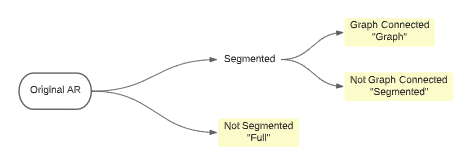
\includegraphics[width=0.8\linewidth]{ThesisFilePkg/figures/data/pipeline.png}
    \caption{The three (in yellow) main feature sets. This AR can either be Segmented or not. When Segmented, it can either be connected in the form of a Graph or not.}
    \label{fig:pipeline}
\end{figure}

After I have extracted the four sub-regions' feature sets, I will create various supervised machine learning models to train on each feature set and compare the results of each model to see if there is an improvement from the Full or SHARPs feature sets. I chose a set of "simple" models (K nearest neighbors, naive Bayes, support vector machine, logistic regression, decision trees, and random forests) and attempted to classify input data points of the vector feature sets as ``M+ flaring" in the next 24 hours or ``M+ quiet" in the next 24 hours. I run each method multiple times and conclude that models trained on the Segmented feature set perform better (an average increase of 0.11 points at best in the True Skill Statistic) than the same models trained on the Full and SHARPs feature sets. I then design an artificial neural network (ANN) to solve my second goal and show that by making minor fixes, I can optimize the model for flare prediction by weighing the importance of ARs closer to flaring in the loss function greater than ARs further from flaring (explained in more detail in chapter \ref{chaptermethods}).

My primary result is that models trained on the Segmented feature set perform better than models trained on either Full or SHARPs. This result satisfies my first goal laid out in the abstract. My second goal will not have any results; instead, I will attempt to explain some of the shortcomings of my models and the problem space as a whole to motivate future efforts in creating a more practical machine learning model to predict solar flares. I conclude that treating this problem as a binary classification problem has its shortcomings and that there are ways to fine-tune models to improve the confidence of short term predictions (and have a higher model performance the closer an input is to flaring).

\chapter{Data and Preliminary Analysis}
\label{chp:data}

\section{Feature Design and Data Description}
\subsection{Raw Data - An AR}
\label{activeregion}
In this thesis, a single AR at some point in time (where $AR^i_t$ is the image of the $i'th$ AR at time $t$) is defined as a collection of a two dimensional continuum array ($C^i_t \in \mathbb{R}^{n\times m}$) and a magnetic field vector field of the same dimensions ($\vec{B} \in \mathbb{R}^{3 \times n\times m}$). These two images both constitute a single AR at a point in time (equation \ref{ardefinition}).
\begin{equation}
AR_t^i := \{C^i_t, \vec{B}\}
\label{ardefinition}
\end{equation}
The dimension $n\times m$ will be used to refer to a single AR dimension in terms of \textit{number of pixel rows} $\times$ \textit{number of pixel columns}; however, ARs vary in size.

I chose the magnetic field because areas of high magnetic flux essentially define ARs. I chose the continuum because it represents more visual aspects of the AR (which have been used extensively for flare forecasting). One AR crossing the face of the solar disk is the object observed inside a \textit{Helioseismic Magnetic Imager AR Patch (HARP)} \cite{HARP} and is a subset of the solar surface that contains strong magnetic fields. The pipeline for extracting ARs is defined extensively in \cite{SHARP_Pipeline}. The Helioseismic and Magnetic Imager (HMI) continuously observes images of the sun and records roughly one terabyte of data every day, including a dopplergram, continuum, line of sight, and vector magnetograms. Although all three data products are helpful, I only use the continuum and magnetogram because these two are the only images I need for the four segments I chose.

The \textbf{magnetogram} is a three dimensional vector field that measures the $x, y, z$ components of the sun's magnetic flux in Maxwells per $cm^2$ ($\frac{Mx}{cm^2}$). The $x, y$ components are the two components tangent to the solar surface, and the $z$ (often called the \textit{line of sight component}) is the magnetic field directed perpendicular to the surface of the sun. Therefore, the measure of magnetic flux must also measure the accumulation (average) flux for each pixel. In practice, JSOC separates the magnetogram into three separate two-dimensional arrays, each of size $n \times m$. 

The \textbf{continuum} is a two-dimensional array (of the same size as the magnetic field components - $n \times m$) that measures the continuum intensity of the solar surface. I chose to include the continuum because primary and reliable modern flare forecasting methods use an AR classification developed by McIntosh et al. \cite{MCintosh} where ``sunspots" (visually dark regions of the sun that are observable by the naked eye) are measured and compared to other sunspots. The local density, spacing, and size of sunspots are all used in the McIntosh scale as shown in figure \ref{fig:mcintoshclass}. 
%%%%%%%%%%%%%%%
\begin{figure}[h]
\centering
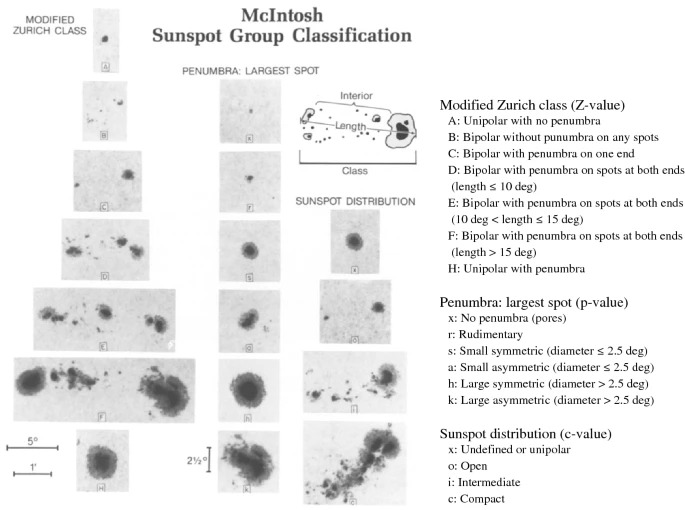
\includegraphics[width=0.5\linewidth]{ThesisFilePkg/figures/data/mcintosh.jpg}
\caption{McIntosh Classification System - measuring the continuum intensity of ARs shows distinct "sunspots" which are regions of \textit{low} intensity. Diagram from \cite{MCintosh}}
\label{fig:mcintoshclass}
\end{figure}
%%%%%%%%%%%%%%
The McIntosh classification system has been used extensively in flare forecasting methods, including Automated Solar Activity Prediction (ASAP, \cite{ASAP}). By including the continuum and magnetogram, I have access to a more general geometry and density measurement than the McIntosh classification system. 

\subsection{Feature Data - Segmentation}
\label{subregions}
 This section will guide the reader through a high level description of the methods taken in order to segment the original AR. Refer to appendix \ref{appendix:algorithms} for a detailed description of the algorithms for each Neutral Line, Umbra and Penumbra segmentation algorithm. 

A Neutral Line is a continuous subset of an AR such that the line of sight magnetic field is $0$ and the gradient from positive to negative is relatively high. In this study, I use the fixed lower threshold of $150 \frac{Mx}{cm^2}$ (both positive and negative), a value chosen by Schrijver \cite{schrijver}). Solar flares frequently occur in these polarity inversion regions. It has been shown \cite{Properties2} that the length of the neutral line with horizontal shear greater than $80^o$ performed well in a one-variable discriminant analysis against flaring and non-flaring ARs. This fact suggests automatically detecting the neutral lines or regions of high magnetic polarity and polarity inversion could be helpful in flare forecasting.

I find Neutral Lines computationally by first thresholding the image, then taking the dilation (an expansion/filling of holes) of positive flux and overlapping this dilation of negative flux to find the intersection of high gradient positive and high gradient negative regions. This step computes where a highly positive region drastically switches to a highly negative region. After finding areas of high gradient and zero magnetic flux, I isolated ``clusters" of the neutral line - which are regions of densely packed zero flux - high gradient polarity inversion lines based on touching pixels - and group these clusters by labeling them by their total area multiplied by their total flux. The result is shown visually in figure \ref{fig:neutralline}.
%%%%%%%%%%%%%%%%%%%%
\begin{figure}[h]
\centering
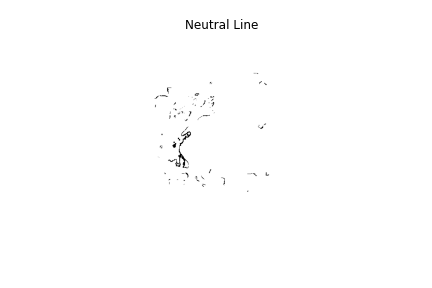
\includegraphics[width=0.5\linewidth]{ThesisFilePkg/figures/data/neutralline.png}
\caption{A neutral line shown visually. On the left is the original line of sight magnetogram; the middle shows the neutral line overlaid on top of the original magnetogram. The right image shows the isolated neutral lines (clustered based on whether pixels are touching).}
\label{fig:neutralline}
\end{figure}

When a high magnetic field exists in the photosphere, the surface traps heat in so-called ``flux tubes". The lower temperature surface ensures a lower intensity, which appears as a black or grey ``sunspot" on the sun's surface. An umbra sometimes has an accompanying penumbra, or secondary low-intensity region, seen as a visually less dark region of the AR but still distinct from the rest of the surface. I found Umbras and Penumbras using mathematical morphology similar to the first method described in \cite{comparisonofumpenmethod} (shown visually in figure \ref{fig:umbra} and \ref{fig:penumbra}).
%%%%%%%%%%%%%%%%%%%%
\begin{figure}[h]
\centering
\begin{subfigure}[b]{0.8\textwidth}
   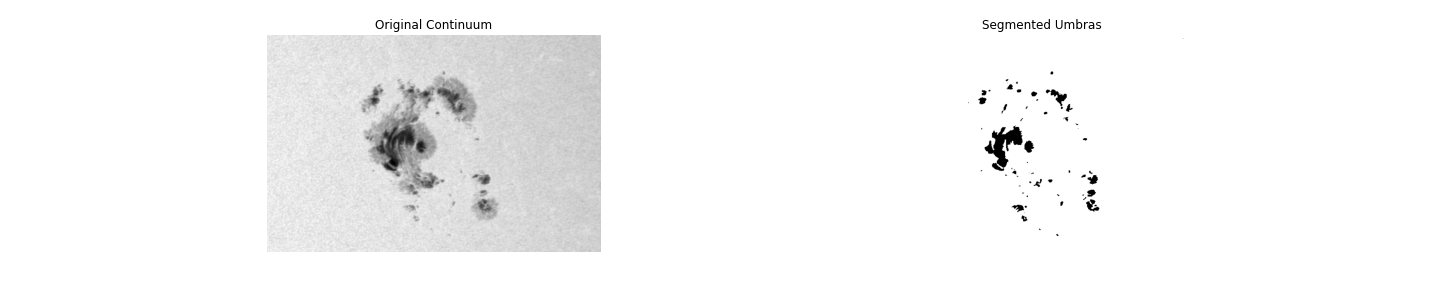
\includegraphics[width=\linewidth]{ThesisFilePkg/figures/data/umbras.png}
   \caption{}
   \label{fig:umbra} 
\end{subfigure}
\begin{subfigure}[b]{0.8\textwidth}
   
\includegraphics[width=\linewidth]{ThesisFilePkg/figures/data/penumbras.png}
   \caption{}
   \label{fig:penumbra}
\end{subfigure}
\caption[Umbra and Penumbra]{(a) An Umbra shown on an AR (shown on the left) and clustered (on the right) based on pixel intersections. (b) A penumbra showed on an AR and clustered.}
\end{figure}

The background is the complement of all other regions. Although not a region used in solar flare forecasting, I include the background to be comprehensive, so I am not ignoring the effects of what is happening just outside of each region. Indeed, if an AR has no neutral lines, umbras, or penumbras, some data should still be collected on this region. Also, I hypothesize that the effects of the magnetogram just outside of each region will affect the future shape and properties of each sub-region. Note that the background is disjoint from all other subsets, the umbra is disjoint from the penumbra, but the neutral line is not necessarily disjoint from the umbra/penumbra.


\subsection{Feature Data - Parameterization}
Recent work (\cite{Properties1} \cite{Properties2} \cite{schrijver}) on characterizing flaring and non-flaring ARs have encouraged the use of scalar parameters based on the physical attributes of the AR. I chose a set of 58 different scalars representing the physical, geometric or statistical properties of subregions of an AR. Some features are multi dimensional. For any of the multiple dimensional features ($X$), I chose to summarize physical quantities using the first four standardized central moments: mean ($\mu$), standard deviation ($E(X - \mu)$), skewness ($E((X - \mu)^2)$), kurtosis ($E((X - \mu)^3)$). I will refer to these four moments as $M(X)$. Some of these formulas require scalar multiples of physical constants, but these will be left out because every quantity is normalized. All 58 features are shown and defined in table \ref{fig:parameters}.
\renewcommand{\arraystretch}{1.8}
\begin{table}[p!]
\centering
\begin{tabular}{||c c c||} 
 \hline
 Property Description & Variable & Formula \\ 
 \hline\hline
 Line of Sight Magnetic Field & $M(B_z)$ & $M(B_z)$\\ 
 \hline
 Total of Magnetic Flux Magnitude & $\Phi_{tot}$ & $\sum_{\Phi \in B_z}|\Phi|dA$ \\
 \hline
 Magnitude of Total Magnetic Flux & $|\Phi_{net}|$ & $|\sum_{\Phi \in B_z}\Phi dA|$ \\
 \hline
 Horizontal Magnetic Field & $M(B_h)$ & $B_h = |B_x| + |B_y|$ \\
 \hline 
 Inclination Angle & $M(\gamma)$ & $\gamma = arctan(\frac{B_z}{B_h})$ \\
 \hline
 $B$ Gradient & $M(\nabla B)$ & $B = |B_x| + |B_y| + |B_z|$ \\
 \hline
 $B_z$ Gradient & $M(\nabla B_z)$ & $M(\nabla B_z)$ \\
 \hline
 $B_h$ Gradient & $M(\nabla B_h)$ & $M(\nabla B_h)$ \\
 \hline
 Vertical Current & $M(J_z)$ & $J_z = \frac{\partial B_y}{\partial x} - \frac{\partial B_x}{\partial y}$ \\
 \hline
 Total of Vertical Current Magnitude & $I_{tot}$ & $I_{tot} = \sum_{j \in J_z}|j|dA$ \\
 \hline
 Magnitude of Total Vertical Current & $|I_{net}|$ & $|\sum_{j \in J_z}dA|$\\
 \hline
 Sum of Each Polarity Current & $|I_{net}^B|$ & $|\sum_{j \in J_z(B_z > 0)}jdA| + |\sum_{j \in J_z(B_z < 0)}j dA|$ \\
 \hline 
 Vertical Heterogeneity Current Density & $M(J_z^h)$ & $(\frac{1}{|B_x| + |B_y| + |B_z|})(B_y \frac{\partial B_x}{\partial y} - B_x \frac{\partial B_y}{\partial x})$\\
 \hline 
 Total of Vertical Heterogeneity Current Magnitude & $I_{tot}^h$ & $\sum_{i \in J_z^h}|idA|$ \\
 \hline
 Magnitude of Total Vertical Heterogeneity Current & $|I_{net}^h|$ & $|\sum_{i \in J_z^h}idA|$ \\
 \hline
 Twist & $M(T)$ & $T = \frac{J_z}{B_z}$ \\
 \hline
 Current Helicity & $M(h_c)$ & $h_c = B_z(\frac{\partial B_y}{\partial x} - \frac{\partial B_x}{\partial y})$ \\
 \hline
 Total of Current Helicity Magnitude & $h_{c tot}$ & $\sum_{h \in h_c}|h|dA$ \\
 \hline
 Magnitude of Total Current Helicity & $|h_{c net}|$ & $|\sum_{h \in h_c}h|dA$ \\
 \hline
 Shear & $M(\Psi)$ & $\Psi = arccos(\frac{\vec{B_p} \cdot \vec{B_o}}{B_oB_p})$ \\
 \hline
 Photospheric excess Magnetic Energy Density & $M(\rho_e)$ & $|B_p - B_o|$ \\
 \hline
 Total Photospheric Excess Magnetic Energy & $E_e$ & $\sum_{p \in p_e}dA$ \\
 \hline
 \end{tabular}
 \caption{A list of all 58 physical scalars currently used by my segmentation method extracted within a subset of an AR and used as inputs to the used machine learning algorithm}
 \label{fig:parameters}
\end{table}

\section{The Three Vector feature sets}
The type, structure, and organization of data in this project will be vital to extracting meaningful results. The intention of the feature extraction of the data collected from the HMI is to be as comprehensive as possible (as many physical features as possible). The three feature sets I will be extracting are theSFull, Segmented, and Graph feature sets. After obtaining a SHARP AR magnetogram and continuum from section \ref{activeregion}, I extracted the three types of segments \textit{without clustering them} as described in section \ref{subregions} (the parameterization of these subsets of the AR is called the Segmented feature set). I will then cluster each subsection into ``nodes" and connect these nodes. This result will be called the Graph feature set.

Since an AR ($AR_t^i$) is a collection of pixels, each with an x, y, z magnetic flux magnitude and a continuum scalar, we can consider the AR as an element of $\mathbb{R}^{4 \times n\times m}$. Let $NL_t^i, UM_t^i, PU_t^i B_t^i\subset AR_t^i$ be subsets of the AR denoting the neutral line, umbra, penumbra and background, respectively. The function $P : \mathbb{R}^{4} \rightarrow \mathbb{R}^{58}$ takes in a subset of the solar surface and computes a vector of many physical features such as total magnetic flux, total shear, etc. 

The Full feature set is expressed in equation \ref{eq:Full} and is simply the physical scalars of the entire AR. This feature set is a control.
\begin{equation}
    D_{\text{Full}} = \{P(AR_t^i) \quad : \quad \forall AR_t^i\}
    \label{eq:Full}
\end{equation}

The Segmented feature set is expressed in equation \ref{eq:Segmented}.
\begin{equation}
    D_{\text{Segmented}} = \{
    \begin{bmatrix}
    \restr{P}{NL_t^i}(AR_t^i) & , & \restr{P}{UM_t^i}(AR_t^i) & , & \restr{P}{PU_t^i}(AR_t^i) & , & \restr{P}{B_t^i}(AR_t^i)
    \end{bmatrix} \quad : \quad \forall AR_t^i \}
    \label{eq:Segmented}
\end{equation}
Where $\restr{A}{B}$ is the restriction of the function $A$ onto the subdomain $B$. The Segmented feature set represents each physical scalar vector for each segment. That is, it is a vector of four stacked vectors, each encoding physical features of their respective subset of the AR.

The Graph feature set is not originally a vector like the other two. I wish to find static properties of individual subsets of the AR and the interaction of one subset with another. This notion of interaction brings to light the idea of a Graph representation, where touching subregions are connected, and nodes on a Graph represent individual regions. The Graph feature set is slightly more complex than the previous two because it requires turning a \textbf{Segmented} AR into a Graph, then turning this Graph into a fixed-length vector.

Given a subset $S \subset AR_t^i$, node $j$ ($S_j$) is a subset of $S$ such that every pixel is touching (equation \ref{eq:touchingpixels}).
\begin{equation}
    S_j, S_k \subset S \qquad S_j \cap S_k = \emptyset \quad j \neq k
    \label{eq:touchingpixels}
\end{equation}
Two nodes $S_j$, $N_j$ (these can be the same or different types) are connected if their intersection of their dilation using a 3x3 kernel is non zero (equation \ref{eq:dilation}).
\begin{equation}
    dilation(S_j, square(3)) \cap dilation(N_j, square(3)) \neq \emptyset
    \label{eq:dilation}
\end{equation}
where the dilation of a region in morphology essentially ``expands and smooths" shapes the set by one pixel (equation \ref{eq:dilationdef}). I use a 3x3 kernel so that each centered active pixel expands one pixel in each direction (that is, a 3x3 kernel expands the set by 1 pixel, a 5x5 would expand it by 2 pixels, a 7x7 would expand it by 3 pixels, etc.):
\begin{equation}
    dilation(A, B) = \cup_{b\in B}A_b
    \label{eq:dilationdef}
\end{equation}
where $A_b$ is the translation of $A$ by $b$. This means that if regions are \textit{bordering} or \textit{intersecting}, they are connected. I chose the one-pixel grouping so that pixels can be a maximum of one pixel from one another. I could use a higher gap; however, this will be a controlled variable for the entirety of the experiment. The connection should measure ``bordering pixels," so the closer the pixels are, the better (and there is no smaller dilation than a 3x3 kernel). For each node, I collect the physical properties using a table of python functions that return the physical quantities described in table \ref{fig:parameters} and tied to that node to create a homogeneous vertex embedded Graph $G$.

\section{Statistical Analysis of the Three Feature Sets}
I designed the problem space to separate ARs into two classes: M+ flaring within 24 hours and M+ non-flaring within 24 hours. It is helpful to look at superficial statistical relationships to see any apparent trends in each feature set. An obvious example is that flaring regions tend to have a higher excess potential energy (often stored in their neutral line). Shown in figure \ref{fig:nlphi}, I observe the distribution of total excess potential energy within the Neutral Line for flaring and non-flaring ARs (left) and the total LOS Magnetic flux (right).
%%%%%%%%%%%%%%%%%%
\begin{figure}[h]
    \centering
    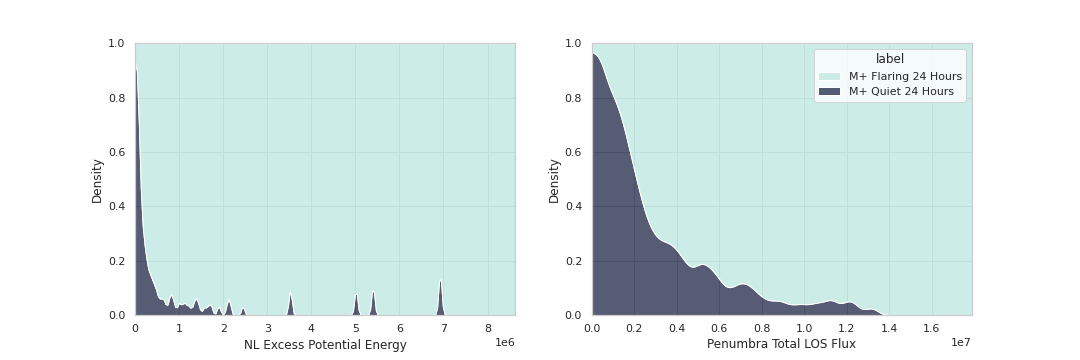
\includegraphics[width=\linewidth]{ThesisFilePkg/figures/data/datasetanalysis.png}
    \caption{KDE Distribution plot of 6601 M+ flaring in 24 hours and 6601 non-flaring ARs. The left plot promisingly shows that most non-flaring ARs had total neutral line potential energy near zero, and most flaring ARs had higher neutral line potential energy. Note that this distribution plot balances the number of flaring and non-flaring data points.}
    \label{fig:nlphi}
\end{figure}
\footnote{These plots are generated by balancing the number of flaring and non-flaring ARs, then creating two histograms. I balanced flaring and non-flaring in this case only to show the difference between the two classes, and the rest of this paper assumes a more realistic ratio of flaring to non-flaring ARs.} The flaring data (light blue) is essentially an inverted density histogram, where each ``bin," or x-axis label sums the percent of ARs that fall in that bin that flare and do not flare to 1. Note that the data comes from a balanced feature set and there are 6601 M+ flaring ARs and 6601 non-flaring ARs in total in the entire plot. So the seemingly dominating upper end of the neutral line potential energy ($\rho$) plot shows that given the neutral line potential energy is immense, the probability of flaring is significant. That is, $p(Flaring \quad | \quad \rho >> 0) \quad > \quad p(Flaring \quad | \quad \rho \quad near \quad 0)$, and a similar statement is made for the distribution of total LOS penumbra flux, but to a lesser degree.

Figure \ref{fig:nlphi} does not necessarily offer a threshold or method to separate flaring/non-flaring regions because some non-flaring regions have a high potential energy of their neutral lines. However, it separates flaring and non-flaring regions in their excess potential energy. In general, the probability that an AR is flaring is higher if it has a higher neutral line excess potential energy for the total flux of the penumbra. This analysis, however, is an observational one, and my feature analysis chapter goes into a more in-depth review of the ranking of features across \textit{all three feature sets}.

\section{Feature Set Limitations} \label{sec:limitations}
\textit{Parameter tuning of the neutral line makes a difference}. In the algorithm to extract the Neutral Line, I use a lower threshold value of $150 \frac{Mx}{cm^2}$ before the positive and negative subsets are dilated and compared. This threshold is an arbitrary number, and some ARs require a higher or lower threshold value. A possible solution to this issue would be to adaptively estimate a threshold value based on the total magnetic flux. For example, use the $60\%$ standard deviation of the total magnetic flux as the lower end threshold. However, this would ignore that some ARs with more neutral lines do not have a higher probability of flaring than an AR with a single, high flux gradient neutral line. I chose a static flux gradient threshold to remain consistent, so the measurement of the geometry and size of the neutral line is maintained. 

\textit{Parameter tuning of the umbra and penumbra makes a difference}. The threshold value of 21000 is chosen arbitrarily from experimentation but removes the accuracy of a human-labeled umbra and penumbra. Typically, umbras and penumbras seem apparent to the observer but are more challenging to segment using an algorithm. A possible solution could include adding a pipeline that extracts umbras and penumbras using computer vision and convolutional neural networks, but this is out of the scope of this study. The library I wrote to extract segments, as it stands, is designed modularly, and changing the algorithm for each segmentation does not ruin the rest of the methods, so I can still do future work to tune the algorithm as it is now.

\chapter{Methods}
\label{chaptermethods}
In this chapter, I will explain the experimental methods I take in order to assess the performance of the Segmented feature set compared to the performance of the Full and SHARP feature set. For my first goal, I will begin by outlining how I will classify models, giving a precise definition for how one model ``performs better" than another and stating the statistical hypothesis test I wish to show. Then, I will explain some of the invalid labelings in my highest performing model (the ANN), and why they may have occurred. I will then describe the precise steps I took in order to optimize the model. Optimizing my highest performing model isn't only about optimizing hyper parameters, it also involves tuning the problem statement itself, i.e what is it I am actually trying to predict? Essentially, how can I design my model to offer the most useful information to solar flare forecasters?

\section{Goal One: Segmentation vs No Segmentation / SHARPs}
I will first show that given a representative subset of machine learning models, models trained on the Segmented features tends to perform better than those trained on the control (Full). 

For the rest of this study, I will utilize a skill score called the true skill statistic (TSS). The TSS uses true positives (TP), true negatives (TN), false positives (FP), false negatives (FN) and finds the true positive and negative rates with respect to total positives and negatives (equation \ref{eq:truerates}). Its meaning and derivation can be found in appendix \ref{appendix:judjingcriteria}. 
\begin{equation}
    TPR = \frac{TP}{TP + FN} \qquad TNR = \frac{TN}{TN + FP}
    \label{eq:truerates}
\end{equation}

Model $M$ is said to perform better on a feature set $D_1 = D_{train1} \cup D_{test1}$ than $D_2 = D_{train2} \cup D_{test2}$ if, after training the model on a training subset $D_{test1} \subset D_1$ that is ``irrelevant" from a testing subset $D_{test1} \subset D_1$, the TSS score of model $M$ on $D_1$ ($TSS(M(D_{test1}))$) is greater than the TSS score on on $D_2$ ($TSS(M(D_{test2}))$):
$$TSS(M(D_{test1})) > TSS(M(D_{test2}))$$
A feature set $D_{test}$ is irrelevant from $D_{train}$ if it is:

\begin{enumerate}
    \item Disjoint from $D_{train}$:
    $$D_{train} \cap D_{test} = \emptyset$$
    \item Has none of the same HARP numbers in either set:
    $$\forall u \in D_{train} \quad (\nexists v \in D_{test} \quad HARP number(u) = HARP number(v))$$
\end{enumerate}

More conditions could be added to this irrelevancy operator, such as avoiding ARs within a certain distance or time of one another. These conditions ensure that we are not overfitting our data on arbitrarily placed training data. That is, we want our model to work for new data, not previously trained data. Also, it is critical that the test feature set models the real world. We can do this by matching a few (2 in this study - the ratio of M and X flares) global metrics that are found in the field with the test feature set. 

Consider a set of ARs that do or do not produce an $M$ or $X$ class flare collected from the Helioseismic magnetic imager over time and the two associated ratios in this feature set:
\begin{itemize}
    \item $\frac{N_x^+}{N}$ - Number of ARs that produce an X class flare ($N_x^+$) over the number of ARs in the feature set ($N$).
    \item $\frac{N_m^+ - N_{mx}^+}{N}$ - Number of ARs that produced only an M flare ($N_m^+ - N_{mx}^+$) over the number of ARs in the feature set ($N$).
\end{itemize}
In the real world, these two ratios vary greatly with time. The roughly 11 year solar cycle shows that flares occur over a pattern of highs and lows. Also, there are other global ratios that are important such as the ratio of $C$, $B$, $A$ class flares to the total number of active regions or the ratio of flares that occur over one section of the sun compared to another section of the sun. Ideally, our test feature set would match all these ratios perfectly; however, in this study, I apply the principle of Randomized Block Design. That is, I have a few known variables (produces M or X class flare) with a known variation and a (theoretically infinite) number of unknown variables with unknown variance (location on the sun, time of year, etc) that I wish to match between our test feature set and the real world, however, I don't have this type of control, so I separate the data by the variables I do know and uniformly sample datapoints from these two blocks so that the other unknown variables are as uniformly distributed as possible. I have calculated the above two ratios and forcefully created the test feature set so that the data points match these ratios. 

From the period of 1996-11-24 17:31:00 to 2018-06-18 8:47:00, there have been a recorded 2015 flaring events of type $M$ and $X$ that range over the NOAA AR numbers 7999-12713. Because NOAA ARs are the input we look at in practice to forecast flares, we will rely on the ratios with respect to the NOAA AR classification convention rather than JSOC's HARP number naming system, although there is very little difference between the two. NOAA ARs are labeled if they are observed by two or more observatories, and are labeled consecutively, so we can estimate there have been a total of $4714 \quad (12713 - 7999)$ ARs that could have been classified in the real world. Note that this time gap is approximately 22 years, which spans approximately 2 solar cycles. This specific date range ensures we are sampling uniformly across solar cycles.

In this time period, there have been 575 NOAA ARs that produced an M flare ($N_x^+$), 78 NOAA ARs that produced an X flare ($N_m^+$), 75 NOAA ARs that produced both X and M flares ($N_{mx}^+$) (showing that most AR's that produce X flares also produce M flares!). So we wish to match the ratios: $\frac{N_x^+}{N} = \frac{74}{4714} = 0.0157$ and $\frac{N_m^+ - N_{xm}^+}{N} = \frac{575 - 75}{4714} = 0.106$. In my feature set, there are 139 SHARPs ARs that produced an M flare, 21 SHARPs ARs that produced an X flare, 13 SHARPs ARs that produced both X and M flares and 739 total SHARPs ARs

To ensure our training to test split is approximately $0.7$, assume we remove $p\%$ of our class $X$ flaring SHARPs and move them to our testing set. Then $N_{x}^+ = 21p$. Now, we also know $N_{mx}^+$ by counting the number of these chosen HARP numbers that also produce $M$ flares. We have two knowns ($N_x^+$, $N_{mx}^+$) and two unknowns ($N_m^+$, $N$). By solving the constraints outlined above (in terms of $p$, and $N_{mx}^+$ is non fixed / randomized):
$$N = \frac{1}{0.0157}N_x^+=\frac{21}{0.0157}p$$
$$N_{m}^+ = 0.106N + N_{mx}^+$$
I wish to make $\frac{N}{739} = 0.7 \rightarrow p = \frac{0.0157*0.7*739}{21} = 0.3867$

Overall, the algorithm to create a train / test split is as follows:
\begin{enumerate}
    \item I take $8$ random X flaring HARP numbers and move them to the test feature set (and all of their associated dates)
    \item Of the $8$ HARP numbers chosen, I count how many of them also produce an $M$ flare and calculate $N_{m}^+ = 0.106*517 + N_{mx}^+$ and take this many ARs from the set of $M$ HARP numbers and move them to the testing feature set.
    \item I fill the rest of the test feature set with non flaring HARP numbers to meet the number of required datapoints in the test set: $N$.
\end{enumerate}
After splitting the data into a train test split where the test data models the real world as best as possible, I train the given model $M$ on the training feature set and compute the $TSS$ (appendix \ref{appendix:judjingcriteria}) score of the test feature set. 

Of course, the results of a single model often vary, so repeating this train / test process is crucial to maximize the benefits of the randomized block design. I repeat for model $M$ 50 times and collect the TSS score for each trial. I now have two iid random variables which have taken the values: $TSS_{D1} = \{tss1_{d1}, tss2_{d1}... tss50_{d1}\}$ and $TSS_{D2} = \{tss1_{d2}, tss2_{d2}... tss50_{d2}\}$. I wish to show that $\bar{TSS}_{D2} \neq \bar{TSS}_{D1}$ with certainty. A two tailed statistical hypothesis can be formulated with the null hypothesis ($H_0$) and alternate hypothesis ($H_A$):
$$H_0: \mu = \bar{TSS}_{D1} - \bar{TSS}_{D2} = 0$$
$$H_A: \mu = \bar{TSS}_{D1} - \bar{TSS}_{D2} \neq 0$$
where $\bar{TSS}$ is the actual (not sample) mean of $TSS$. Using a $z-test$ because $n > 30$, I use the $\alpha = 0.01$ level threshold to confidently say that the $TSS$ score produced by feature set 1 ($D1$) is different than the $TSS$ score produced by feature set 2 ($D2$), and I simply order the two by rank. If $TSS_{D1} > TSS_{D2}$ then $D1$ performs better under model $M$ than $D2$. 

% Model classes - p test etc / trials
\subsection{Ranking Models}

The notion of ranking a model by its performance, I found, can be used to separate models into three specific classes (for comparing against both the Full and SHARPs feature set):

\begin{itemize}
    \item Class 1: $TSS(Segmented) > TSS(Full / SHARPs)$
    \item Class 2: $TSS(Segmented) = TSS(Full / SHARPs)$
    \item Class 3: $TSS(Segmented) < TSS(Full / SHARPs)$
\end{itemize}

Note that if $p > \alpha$, then the model belongs to class 2, but if $p < alpha$, the model could belong to either Class 1 or 2 depending on the ranking of scores. To rank a model $M$, it is important that $M$ must be maximized \textit{with its own feature set} as best as possible. That is, the parameters of $M$ change significantly between the Full and Segmented feature sets. For example, a value of $k = 101$ neighbors worked best for the Full feature set and a value of $k = 81$ neighbors worked best for the Segmented feature set. The models used in this study are chosen as high level, widely used models including (each with optimized parameters) K Nearest Neighbors, Randomized Forest, AdaBoost, Support Vector Machine, Decision Trees, Naive Bayes, Logistic Regression, and an ANN. 


\section{Goal Two: Analyzing the Best Performing Model}
I was interested in diving deeper into the process of how the model worked and failed in the ANN. First, I wanted to find out \textbf{why certain points missed}. For each of the trials I conducted on the ANN, I labeled each data point as a $TP$, $TN$, $FP$, or $FN$, and kept track of how many of each of these classifications each data point was labeled as. I analyzed each of these metrics with respect to \textit{flare class} and \textit{hours until flaring}.

I also performed a feature selection on all features combined across all three feature sets and examine the highest performing features overall. If one feature set tends to dominate, then we can safely assume that this feature set is more ``informative". Because this problem is inherently nonlinear, simple statistical analyses such as ANOVA or F-distributions won't work well. It is surely possible that some parameters are linearly separated, but a nonlinear correlation statistic is used called the Kendall rank correlation coefficient test, which is a more general form of the general correlation coefficient. 

Finally, I present and briefly describe the results a proposed model that incorporates fixes to the problems that I summarized in the previous paragraph. This model is a multi step regression problem that incorporates A, B, and C flares as well as M and X flares and creates a regression on time till flare and flare magnitude.

\section{Models}

In order to rank the general effectiveness of a single feature set, I compare the feature set performance on a wide variety of models including simple ones such as K nearest neighbors and Random Forests, as well as more sophisticated models including Logistic Regressions and ANNs.

I test each model on the Full feature set as well as a dimension-reduced feature set of 10 of the most prominent features. This is to remove ``curse of dimensionality" bias for certain models. For example, in K nearest neighbors, it is well known that the error often scales with the dimensionality of the input space. 

Also, for each (simple) model, I utilize Scikit-Learn's Grid Search functionality to optimize hyperparameters. For the ANN and more complex variations, it is not possible to run through various network topologies / hyperparameters, so I utilize one neural network, while acknowledging that it may be possible to increase the score by changing the network topology and optimizing hyperparameters.

\subsection{Simple Models}

For this experiment, I have chosen six primary simplistic models, which allows me to understand some of the properties of each feature set. Testing simple models allows me to make a more general conclusion that most (at least all the ones that I have tested on) machine learning methods perform better on my Segmented feature set than others. Each model is trained and optimized using a grid search algorithm \textit{for the individual feature set}. Therefore, hyperparameters vary between each feature set that give the best possible score for each feature set. This is meant to simulate true machine learning, where only the most optimal model would be considered, and the subsequent best hyperparameters are used. The models I use with optimized hyper parameters for each feature set are shown in figure \ref{tab:hyperparameterssmall}.
\begin{table}[p]
    \centering
    \begin{tabular}{|p{0.2\linewidth}|p{0.25\linewidth}|p{0.25\linewidth}|p{0.25\linewidth}|}
        \hline
         \textbf{Model Name} & \textbf{Segmented Hyperparameters} & \textbf{Full Hyperparameters} & \textbf{SHARPs Hyperparameters} \\
         \hline
         Random Forest (RF) & Max Depth = 11 & Max Depth = 7 & Max Depth = 3 \\
         \hline
         K Nearest Neighbors (KNN) & k = 101 & k = 51 & k = 41 \\
         \hline
         Naive Bayes (NB) & N/a & N/a & N/a \\
         \hline
         Support Vector Machine (SVM) & Radial Basis Function Kernel & Radial Basis Function Kernel & Radial Basis Function Kernel \\
         \hline
         AdaBoost & Number of Estimators = 60, learning rate = 0.1 & Number of Estimators = 40, learning rate = 0.5 & Number of Estimators = 30, learning rate = 0.5\\
         \hline
         Decision Tree & N/a & N/a & N/a \\
         \hline
         Logistic Regression & L2 penalty & L2 penalty & L2 penalty \\
         \hline
    \end{tabular}
    \caption{All of the hyperparameters \textit{that I grid searched} for each model for each feature set. Note that there may be more features hyperparameters that were not optimized.}
    \label{tab:hyperparameterssmall}
\end{table}

\subsection{ANN}
The Artifical Neural Network topology (number of nodes, hidden layers etc.) is kept the same on all three feature sets. The model is a sequence of three layers, consisting of an input layer, a 32 dimensional layer, a 12 dimensional layer and an 8 dimensional layer. On each layer, there is a dropout module with $p = 0.5$ and a RELU activation function. Weights are initialized via the Xavier Normal initialization algorithm. I used AdaGrad optimization algorithm with weight decay equal to $0.1$ and learning rate equal to $0.005$. I ran 50 epochs for each feature set and observed for effects of overfitting but this was not an issue. This full architecture is shown in figure \ref{fig:ann}.
\begin{figure}[h]
    \centering
    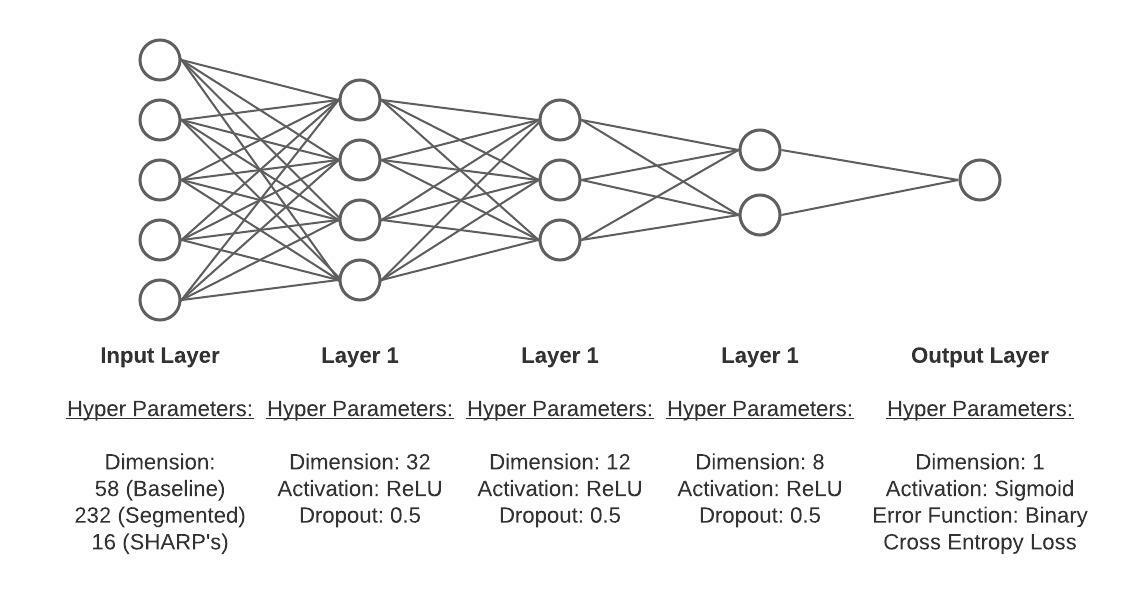
\includegraphics[width=\linewidth]{ThesisFilePkg/figures/methods/ann.jpeg}
    \caption{The ANN Design}
    \label{fig:ann}
\end{figure}

Due to the heavily unbalanced feature set, in my training data, I weighted flaring data points as 100 and non flaring data points as 10 in my binary cross entropy loss function. I also decreased the weights of ARs near the 24 hour mark using the relationship in equation \ref{weight}. Each AR data point is assigned a value of $t$. For flaring ARs, this is simply the time until the next M+ flare. For non flaring regions, $t$ is treated as infinite and the weight is taken as $t \rightarrow \infty$. I assign an asymptotic flaring weight ($a_f = 10$) and an asymptotic non flaring weight ($a_{nf} = 100$) that each describe the extremes of flaring and non flaring regions to my model (ie $t = 0$ and $t \rightarrow \infty$). I have a minimum weight ($w_min = 0.1$) equal to the weight of an AR that would occur in exactly 24 hours and two scaling terms: $a = 1$, $b = 30$ that scale the curvature of the climb of both flaring and non flaring weights, respectively. 
\begin{equation}
    weight(t) = 
    \begin{cases}
        (a_f - w_{min})(1 - e^{-\frac{(t - 24)^2}{24a}}) + w_{min} \quad t \in (0, 24]\\
        (a_{nf} - w_{min})(1 - e^{-\frac{(t - 24)^2}{24b}}) + w_{min} \quad t \in [24, \infty)
    \end{cases}
    \label{weight}    
\end{equation}
and the distribution of weights with respect to time till flare is shown in figure \ref{fig:weights}.
\begin{figure}[h]
    \centering
    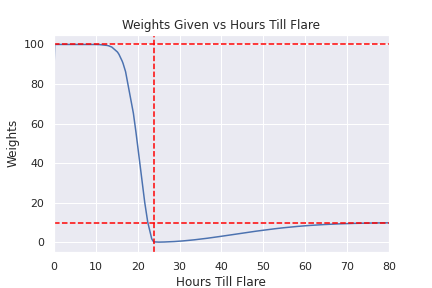
\includegraphics[width=0.5\linewidth]{ThesisFilePkg/figures/methods/weights.png}
    \caption{The weights assigned to each AR data point given its time till flare in the Binary Cross Entropy Loss Function. Non flaring ARs are taken as $t \rightarrow \infty$. The left hand asymptote (top red line) is 100, the right hand asymptote (bottom red line) is 10 and the minimum weight (middle vertical red line) is 0.1.}
    \label{fig:weights}
\end{figure}

\subsection{Graph Models}
For my Graph feature set, I need to first represent each Graph as a vector (through a node embedding), then pass this vector into the same (optimized) models described above. This simplifies the process of comparing the performance of a model on Graph feature set by using the same models with that added step of node embedding. I tried two methods of node embeddings: a Graph neural network autoencoder and node2vec. I found that node2vec had too many parameters to tune (in addition to the massive amounts of parameters to tune in the feature extraction algorithm itself), which made it unwieldy for the hundreds of thousands of data points I had access to.

An autoencoder is designed to take in an input, and transform it in some way to a low dimensional fixed vector space by an encoder layer then decodes the vector into the input data format with a minimal amount of error between the initial input and decoded output. Let the original Graph $G$ be a collection of nodes $v$ (a 58-dimensional vector representing all the physical features of that node) and edges $e$ (that connect two nearby nodes).  The Graph neural network takes the neighbors of each node $v$ ($n(v)$) and  transforms them into a new space. After transformation, the new vector $v\prime$ becomes:

$$v'= \sigma (W*v + \sum_{n(v)} W*n(v))$$ 

Where $\sigma$ is some activation function (I used ReLU), and $W$ is a  learn-able weight matrix. This transformation is done for each node in the Graph, and the same transformation is applied to the neighbors of $v$. This process can be repeated multiple times (according to the number of Graph layers). I chose only one layer. 

The final Graph $G'$ is a transformed version of the original Graph $G$ with the same topology, only the original vectors $v$ are represented as transformed vectors $v'$. Then, I take the average of all nodes as the final vector encoding. This vector is supposed to represent all aspects of the Graph including the Graph topology and vector values of each node. The decoder takes in this vector and predicts a theoretical new Graph ($\hat{G}$) including both topology and node values that is ideally exactly the same as Graph $G$. The error between the two Graphs represents the machine learning loss function and is taken as the Graph edit distance (GED) plus the difference in average nodes:
\begin{equation}
    d(G, \hat{G}) = GED(G, \hat{G}) + |\frac{1}{N}\sum_{v \in G}v - \frac{1}{\hat{N}}\sum_{\hat{v} \in \hat{G}}\hat{v}|
    \label{graphmetric}
\end{equation}
Equation \ref{graphmetric} is the sum of the distance \textit{in topology} and the difference \textit{in average node embeddings} of the graph, meaning it takes topological, geometric and physical error into account.

The final vector could then be used in all the previously mentioned models, however, I chose to only test this vector embedding on the ANN. This is because, although the idea of Graph encoding could work for detailed Graphs representing each AR, a majority of Graphs in my feature set were seemingly invalid. Many Graphs had no nodes at all (a small amount of which surprisingly flared in 24 hours), and many Graphs were composed of disjoint Graphs. This means that the Graph embedding step would label all no-node Graphs the same (flaring or not), and would struggle to find any sort of relationship between nodes that weren't connected to one another (because there would be no update step in the primary Graph neural network step that encodes the Graph into a vector). I will share my results for this model in the findings chapter, but they should not be taken significantly because of the previously mentioned issues.


\subsection{Other Models}

The above models were compared between Full and Segmented (with the exact algorithm explained below). I was also interested in changing the problem space to find the most optimal model. I tried various other models including ones that used time series analysis on the data. I created a \textbf{time stacked} neural network, where I took the 10 most important features, and stacked vectors with a distance of $s$ hours from one another and overall lookback of $l$ (meaning a total hour look back of $s \times l$). Data were considered $batch \times lookback \times 10$ dimensional input vectors and passed to the neural network as is. 

I also designed an LSTM binary classifier, ANN Regression model, LSTM Auto Encoder and ANN Auto Encoder, but I will not be considering the results of these models for the scope of this study.

\chapter{Findings}

\section{Goal one: Segmentation vs No Segmentation / SHARPs}
\subsection{Model Rankings}

After training and testing the seven simple machine learning models and the ANN described in the previous chapter, all methods, except random forest and decision trees, performed better when trained on the Segmented feature set than on the Full and SHARPs feature sets. Although the Random Forest and Decision tree performed better more often when trained on the Segmented feature set in the trials I ran, the resulting difference in the means of the TSS scores between the three feature sets for these two models was not big enough to warrant a rejection of the null hypothesis that the two models performed the same. This failure of rejection is likely due to the significant standard deviation of scores of these two models. Recall that I define class 1 models as those that perform better on the Segmented feature set than on the Full and SHARPs feature sets and class 2 models as those that perform equally between all three feature sets. Figure \ref{tbl:bsseg} shows the resulting classes for each model comparing the Segmented and Full trained models, where the p-value indicates the statistical certainty that a model belongs to a particular class (a lower p-value is a more specific result). I use a statistical test at the $\alpha = 0.01$ level to show that a model belongs to a particular class. That is:

\begin{itemize}
    \item If $p < \alpha$, then $TSS(Segmented) \neq TSS(Full/SHARPs)$ - Class 1 or 3
    \item If $p \geq \alpha$, then $TSS(Segmented) = TSS(Full/SHARPs)$ - Class 2 
\end{itemize}

\noindent Figure \ref{tbl:shpseg} shows the same table comparing the SHARPs and Segmented trained model.

\begin{table}
\begin{center}
\begin{tabular}{c|c|c}
     Method & $P(\bar{TSS}(Full) \neq \bar{TSS}(Segmented))$ & Class \\
     \hline
     K Nearest Neighbors & 2.1e-12 & Class 1 \\
     Naive Bayes & 4.5e-16 & Class 1 \\
     Decision Tree & 0.04 & Class 2 \\
     Random Forest & 0.16 & Class 2 \\
     AdaBoost & 3.9e-5 & Class 1 \\
     Support Vector Machine & 3.0e-5 & Class 1 \\
     Logistic Regression & 3.2e-8 & Class 1 \\
     ANN & 1.1e-12 & Class 1
\end{tabular}
\caption{Comparing the results of 50 trials of each method optimized and run on the Full and Segmented feature sets. A low p value indicates that it is very likely that the actual mean score of the Segmented feature set is different than the actual mean score of the Full feature set. Class 1 methods performed better on the Segmented feature set than the Full and class 2 methods performed equally on both feature sets.} 
\label{tbl:bsseg}
\end{center}
\end{table}

\begin{table}
\begin{center}
\begin{tabular}{c|c|c}
     Method & $P(\bar{TSS}(SHARPs) \neq \bar{TSS}(Segmented))$ & Class \\
     \hline
     K Nearest Neighbors & 1.1e-8 & Class 1 \\
     Naive Bayes & 5.6e-12 & Class 1 \\
     Decision Tree & 0.02 & Class 2 \\
     Random Forest & 0.03 & Class 2 \\
     AdaBoost & 3.5e-12 & Class 1 \\
     Support Vector Machine & 7.1e-7 & Class 1 \\
     Logistic Regression & 1.8e-8 & Class 1 \\
     ANN & 1.9e-5 & Class 1
\end{tabular}
\caption{Comparing the results of 50 trials of each method optimized and run on the SHARPs and Segmented feature sets. A low p value indicates that it is very likely that the actual mean score of the Segmented feature set is different than the actual mean score of the SHARPs feature set. Class 1 methods performed better on the Segmented feature set than the SHARPs and class 2 methods performed equally on both feature sets.} 
\label{tbl:shpseg}
\end{center}
\end{table}

None of the methods I found fell in Class 3 for Full or SHARPs feature set comparison, promising for the Segmented feature set. The majority of methods performed the best on the Segmented feature set, which implies that most machine learning models perform better when trained on the Segmented feature set, and if anything, a select few less accurate machine learning models perform the same between all three feature sets. Notably, the best results came from the ANN, and this model performed far better when trained on the Segmented feature set than the other two feature sets (with an average $TSS$ score of $0.787 \pm 0.05$ when trained on the Segmented feature set, an average $TSS$ score of $0.759 \pm 0.04$ when trained on the Full feature set, and an average $TSS$ score of $0.676 \pm 0.06$ when trained on the SHARPs feature set). 

We see two primary results. First, models trained on the Segmented feature set perform better than those on the Full feature set, which means that the added segmentation step increases the amount of helpful information for machine learning models. This assertion is supported when we take a dimension reduction of both feature sets to only focus on the top 10 features alone. When I measured the shared information (discussed precisely in my feature selection section), I took the top 10 most important features of the Segmented and Full feature sets. I then trained the same model on both of these ten features. Again, the ANN model performed better on the Segmented feature set than the Full feature set (with a p-value of 1e-12), which means that each feature of the Segmented feature set contains more information than the Full feature set, and it is not just the fact that there are more features in the Segmented feature set than the Full that models trained on the Segmented feature set perform better.

Second, models trained on the Segmented feature set perform better than those on the SHARPs feature set, which means that the Segmented feature set increases the amount of helpful information for machine learning models compared to a controlled standard. The same feature reduction method was used, and models trained on the Segmented feature set still performed better (with a p-value of 2e-6).  

\section{Goal two: Analyzing the Performance of the ANN}
I analyze the false rates for certain flaring classes and time ranges to find which active regions tend to fail. The false positive rate (FPR) is defined as the ratio of false positives over total negatives and the false negative rate (FNR). These two rates are shown in equation \ref{eq:falserates}.

\begin{equation}
    FPR = \frac{FP}{FP + TN} \qquad FNR = \frac{FN}{FP + TN}
    \label{eq:falserates}
\end{equation}

\subsection{Fixing the False Rates and Problem Space}
We find that X flaring ARs were falsely predicted as negative far less than M flaring ARs, which indicates that magnitude should be considered in the output variable of the problem space. Figure \ref{fig:segfnr} shows the false negative rates of the ANN when trained on the Segmented feature set and tested on a disjoint testing set. The x-axis indicates the type of flare that occurred, and the y-axis indicates time bins for the time until flaring. For example, of the tested ARs that produced an M flare between 2.415 and 4.813 hours, the false-negative rate for this specific subset was 0.024. We see X-flaring ARs had a 0 false-negative rate between those that flared in 0-19.203 hours and a low false-negative rate for those between 19.203-24 hours. In each time bin, ARs that produced an M flare had a higher false-negative rate than those that produced X flares. So M flaring ARs were falsely labeled negative more frequently than X flares.
%%%%%%%%%%%%%%%%%%%%%%%%%
\begin{figure}[h!]
    \centering
    \includegraphics[width=0.6\linewidth]{ThesisFilePkg/figures/findings/SegmentedFNR.png}
    \caption{The false-negative rates for ARs that flared within h hours (where h is found in either time bin on the left axis) for class M and X flares, respectively. Notice that X flaring regions' false negative rates are 0 from 0 hours to 19.203 hours but spike near the 24-hour mark. The same can be said for M flaring regions, which show a significantly higher false-negative rate.}
    \label{fig:segfnr}
\end{figure}

We also find that X flaring ARs were falsely predicted as positive far more often than M flaring ARs, which again indicates that magnitude should be considered in the output variable of the problem space. Figure \ref{fig:segfpr} shows the false-positive rates for ARs \textit{that produced a flare within 24 hours}. Recall that our model was a binary classification, with a threshold of 24 hours for flaring and non-flaring. So an AR could have flared within 24 hours and been treated as a negative. Notice that of all the time bins, X flaring ARs had a higher false-positive rate than M flaring ARs. 
%%%%%%%%%%%%%%%%%%%
\begin{figure}[h!]
    \centering
    \includegraphics[width=0.6\linewidth]{ThesisFilePkg/figures/findings/SegmentedFPR.png}
    \caption{The false-positive rates for ARs that flared within h hours (where h is found in either time bin on the left axis) for class M and X flares, respectively. Notice that except for the last two data points of the x flare, the false positive rate is highest for both M flares and X flares closer to 24 hours as expected and that in general, false-positive for X flaring ARs is less than the false positive rate of M flaring regions.}
    \label{fig:segfpr}
\end{figure}

The previous two findings indicate that the magnitude of flare is an important characteristic that should be captured in the output variable. We cannot just label flaring and non-flaring ARs because some flares are more significant than others, which should be captured in the output. The false-positive and negative rates for the Full and SHARPs feature sets are shown in appendix \ref{appendix:fprfnrother}

From figures \ref{fig:segfnr} and \ref{fig:segfpr}, we find that false rates are higher the closer the AR is to 24 hours. As the y axis approaches 24 hours (the bottom of the chart in figure \ref{fig:segfnr} and the top of the chart in figure \ref{fig:segfpr}) the false rates grow for both M and X flaring regions. Intuitively, this makes sense because, for example, if we look at an AR that flares in 23.9 hours, and one that flares in 24.1 hours, both would look very similar (they are only separated by 12 minutes, so not much could have changed in the AR). However, these two ARs are labeled differently. I attempted to fix this problem in my weighting of the Binary Cross Entropy Loss Function shown in figure \ref{fig:weights} by weighting the importance of incoming data that were closer to the 24-hour mark, but the issue persists. This finding indicates that the time until the flare is an important characteristic that should be captured in the output variable of the machine learning model. We cannot simply label an AR as flaring or non-flaring; we also need to label the time until the flare happens.

These two problems, that the magnitude and time are two important characteristics that should be captured in the output variable, can be fixed in two ways. Either change the problem to a regression one or add in overlapping ``bins" to increase the categorical classification of flares. In both these solutions, we are increasing the possibilities of the output space to include the different magnitude and timed flares. 

I implemented the first solution and changed the problem to a regression one, which is possible due to the fact that I can use a threshold a regression problem to turn it into the exact same binary classification problem as before. In this newly proposed problem space, rather than a model that predicts M+ flaring in 24 hours, we create a real-valued machine learning model that takes in an AR and returns the time and magnitude of a flare:

$$f_{regress} : AR \rightarrow (t, M)$$

\noindent where $t$ is the time until flare and $M$ is the magnitude of the flare. A problem arises: how do we label non-flaring ARs (that never flare)? There are a few solutions to this problem that are arbitrary in their own way. I chose to label all non-flaring regions with the time of two weeks (336 hours) and 0 magnitude. Then, I took all flaring ARs and changed the time until flare to two weeks. Two weeks is chosen because it is large enough to capture information for 24 hours. Suppose we create a regression problem and note if an AR flares within 24 hours; this is essentially the same classification problem as before. The magnitude implies that we also need to label more minor flares (both to capture more information and be more complete in our output). Solar flares are labeled with a letter (A, B, C, M, X) followed by a number greater than or equal to one and strictly less than 10. The number following the letter tells the factor of strength the flare is from the Full. An $A5$ flare is $5$ times greater than an $A1$ flare. $A$ flares are all those with peak flux at 0.1-0.8 manometer X-ray range less than $10^{-7}$. $B$ flares have a peak flux from $10^{-7}-10^{-6}$. $C$ flares have a peak flux from $10^{-6}-10^{-5}$. $M$ flares have a peak flux from $10^{-5}-10^{-4}$. $X$ flares have a peak flux greater than $10^{-4}$. I labeled AR magnitude with approximate magnitude inferred from their class labels. 

I created the same ANN as before, only changing the output variable to two real values indicating the time and magnitude of flare. I labeled each data point with its magnitude and time till flare, setting non flaring ARs $(t, M) = (336, 0)$ and all ARs with $t > 336$ to $t = 336$. I added a final threshold to the output for the time and magnitude so that if the output time was less than 24 hours and the magnitude was greater than $10^{-5}$, the label was treated as positive, and all other outputs were treated as negative. The resulting $TSS$ score for 5 of these train/test cycles came out with a mean of $0.754 \pm 0.01$, which is less than the achieved score of $0.787$ achieved by the simple binary classification problem. There are a few reasons the regression problem could have performed worse. First, regression problems are inherently more challenging to train with a small feature set. If I had more data points, the regression problem could have performed better, but I have no way of knowing yet, and with the data, I have now, the binary classification performed the best.

\subsection{Feature Ranking}
To assess the importance of each feature, I used a mutual information test. Mutual Information (equation \ref{eq:mutualinformation}) between two random variables, X (the feature) and Y (M+ Flare within 24 hours), is a metric that assesses how independent the two random variables are. It measures the joint pdf $p_{X,Y}(x, y)$ and marginal pdfs $p_X(x)$ and $p_Y(y)$ and compares them.
\begin{equation}
    I(X, Y) = \sum_{x \in X}\sum_{y \in Y}p_{X,Y}(x, y)log(\frac{p_{X,Y}(x, y)}{p_X(x)p_Y(y)})
    \label{eq:mutualinformation}
\end{equation}
where $I(X, Y) = 0$ if X and Y are independent. Therefore, higher mutual information means a certain feature $X$ can be associated with flaring / non-flaring $Y$. 

It was observed that most of the highest mutual information features were from the Segmented feature set. The highest feature was the total excess potential energy of the neutral line (nl\_totrho). The ordering of the top 15 Mutual Information scores for each of the feature sets are shown in figure \ref{tbl:ftrank}.
%%%%%%%%%%%%%%%%%%%%%%%
\begin{table}
\begin{center}
\begin{tabular}{c|c|c}
     Variable Description & Mutual Info & From feature set \\
     \hline
     Total Neutral Line Excess Potential Energy & 0.0806 & Segmented \\
     Total unsigned current helicity & 0.0721 & SHARPs \\
     Total sum of vertical current within the Penumbra & 0.0701 & Segmented \\
     Total sum of horizontal current within the Penumbra & 0.0701 & Segmented \\
     Total sum of horizontal current within the neutral line & 0.0688 & Segmented \\
     Total sum of current helicity within the penumbra & 0.0682 & Segmented \\
     Standard deviation of excess potential energy in the penumbra & 0.067 & Segmented \\
     Total unsigned vertical current & 0.0669 & SHARPs \\
     Total sum of vertical magnetic field within the penumbra & 0.0650 & Segmented \\
     Total sum of the magnitude of current helicity in the penumbra & 0.0635 & Segmented \\
     Total sum of the magnitude of current helicity in the neutral line & 0.0631 & Segmented \\
     Sum of the magnitude of the net currents & 0.0629 & SHARPs \\
     Total Excess Potential Energy & 0.063 & SHARPs \\
     Total sum of the magnitude of current helicity & 0.0621 & Full \\
     Total sum of current helicity within the umbra & 0.0618 & Segmented
\end{tabular}
\caption{Feature Ranking of all Features stacked together using the Kendall-$\tau$ statistical correlation test.} 
\label{tbl:ftrank}
\end{center}
\end{table}

Figure \ref{tbl:ftrank} shows that the ANN likely did not only perform better when trained on the Segmented feature set than the other two feature sets because it had more features; likely, each individual Segmented feature held more significance than both other feature sets. The top 15 features included 10 Segmented features, 4 SHARPs features, and 1 Full feature. When I trained the ANN on only the ten most important features of each feature set, I found that the ANN performed worse when trained on Full than SHARPs, even though it performed better when trained on all the features of the Full feature set. I hypothesized that the Full feature set only performed better because it had more features. The results in figure \ref{tbl:ftrank} support this conclusion because only one Full feature captured enough mutual information to belong to the top 15 features compared to 4 SHARPs features. When I did the same test between Segmented and SHARPs and reduced the number of features to the top 10, the ANN trained on the Segmented feature set performed better than the ANN trained on the SHARPs feature set. This fact, along with the fact that the Segmented feature set has ten features on table \ref{tbl:ftrank} while the SHARPs feature set only had four, indicates that it performed better because individual Segmented features held more importance than those of the SHARPs features. 


\section{Graph Results and Discussion}

The model results described in my methods section applied to the Graph feature set were underwhelming. The TSS score for the Graph feature set was $0.454 \pm 0.04$. Some possible reasons for the poor performance include the fact that there were far too many parameters to tune in the Graph segmentation algorithm, including the number of nodes, number of nodes to keep, what constitutes a connection, and other high-level aspects of the Graph algorithm, which require me to recompute the feature set many times, which is not reasonable with the amount of time it takes (being roughly two-three weeks of processing time). Another potential reason for the poor performance of the algorithm is that the feature set itself may be too noisy. 

Despite the poor TSS score, I believe there is potential to improve in the future. This feature set is a helpful tool for the solar physicist because the feature set offers a general way of measuring how specific regions of an AR are related to one another. This can give us insight into how the solar magnetic field is structured and how that structure might influence the production of flares. 

\chapter{Conclusions}

There were three main conclusions drawn that support the use of the Segmented feature set for flare forecasts. First, I showed that a large selection of machine learning models of various complexity perform better in M+ solar flare forecasting within 24 hours when trained on the new Segmented feature set than the same models trained on the Full. This shows that the extra segmentation step proposed in this work does improve the performance of machine learning models for solar flare forecasting. Second, I showed that the same models also performed better on the Segmented feature set compared to those models trained on the SHARPs feature set, which shows that the Segmented feature set generally offers more information than a widely used feature set in solar flares studies. This can have significant implications since the segmentation step proposed in this work offers improved performance in forecasting and provides new insights that were not possible to obtain with the Full feature set. Third, I all models on dimension reduced versions of each feature set, and the same results applied, meaning that not only did the feature set as a whole offer more information to machine learning models, but individual features alone in the Segmented feature set were more informative to flaring / nonflaring than SHARPs features and Full features. Overall, these three observations show that the segmentation step proposed in this work offers a significant improvement in performance for solar flare forecasting with machine learning models and new insights into the behavior of solar flares. 

There were not any robust conclusions I could draw that support the use of the Graph feature set, other than suggestions. I showed that the Graph feature set did not perform well in automated flare forecasting with machine learning and that, in its current state, it should only be used as a supplement to other data. This lack of performance came from the fact that there were so many parameters to tune and edge cases to test in the Graph feature set, as it is now that some resulting Graphs were widely misunderstood by the present encoding algorithms I tried to use.  

In the future,  I plan to extend this work by incorporating additional data sources such as Helioseismic and Magnetic Imager (HMI) vector magnetograms and Solar Dynamics Observatory (SDO)/AIA images to improve performance further. Additionally, I plan to develop new Graph-based features that can be extracted from the HMI and SDO/AIA data to improve the performance of the Graph-based approach. 

%%%%%%%%%   then the BiblioGraphy, if any   %%%%%%%%%
\bibliographystyle{plain}	% or "siam", or "alpha", etc.
\nocite{*}		% list all refs in database, cited or not
\bibliography{refs}		% Bib database in "refs.bib"

%%%%%%%%%   then the Appendices, if any   %%%%%%%%%

\appendix


\chapter{Segmentation Algorithms}
\label{appendix:algorithms}

\section{Penumbra and Umbra Extraction}
The \textit{Umbra} and \textit{Penumbra} are distinctly dark spots on the continuum. When the photosphere has an abnormally high magnetic field, heat is trapped beneath the surface. The lower temperature surface ensures a lower intensity, which appears as a black or grey ``sunspot" on the surface of the sun. An umbra sometimes has an accompanying penumbra, where the continuum shows a secondary low intensity. The penumbra is seen as a visually less dark region of the AR, but still distinct from the rest of the surface. We find Umbras and Penumbras using mathematical morphology and adaptive thresholding. These distinct regions are shown visually in figure \ref{fig:binarythresh}.

First, we extract the Umbra and Penumbra in the same algorithm. This is because the Umbra and Penumbra are very closely tied to one another. A few high level axioms guide our thinking. First, Umbra and Penumbra are darker \textit{than their surroundings}, but regions further from an Umbra may be just as dark. Therefore, rather than threshold the image as a whole, we use a localized adaptive filter that thresholds the image using localized grids. Second, a group of ``dark" pixels (low intensity) can either be unimodal (only an Umbra) or bimodal (an Umbra with an accompanying Penumbra). 

The algorithm to extract Umbras and Penumbras is shown in \ref{alg:umpum}:

\begin{enumerate}
    \item First, (lines 3-6) we bound the continuum intensity from 0 to 255. The absolute magnitude of the continuum shouldn't matter because an Umbra and Penumbra is simply a darkened region compared to their surroundings. A binary adaptive threshold \cite{scikit} takes into account that there may be shadows or dark regions in the image that are not necessarily Umbras or Penumbras. For example, in figure \ref{fig:binarythresh}, the right side of the original continuum is darkened due to a shadow, which could interfere with a global threshold. The binary adaptive threshold only considers localized kernels (in this case, we restrict the filter to a 5x5 kernel, which is chosen through experimentation, but is a parameter the user can adjust if they see fit). Each threshold is the weighted mean of the local neighborhood. After we threshold, this leaves us with a binary array showing regions that are greater than (false) or less than the adaptive threshold value (true). The output of this step is shown in figure \ref{fig:binarythresh}. Now, this whole region is set equal to the Umbra:
    
    $$Umbra \gets binaryAdaptive(C)$$
    
    and in step two, I subtract the Penumbra from the previously defined Umbra:
    
    $$Umbra \gets Umbra \cap \neg Penumbra$$
    
\begin{figure}[h]
\centering
\begin{subfigure}[b]{.45\textwidth}
  \centering
  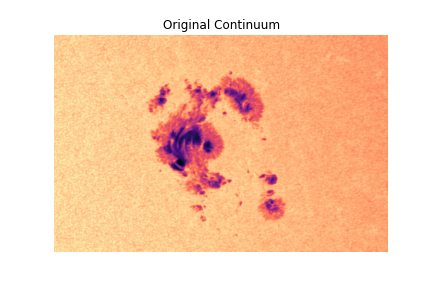
\includegraphics[width=.8\linewidth]{ThesisFilePkg/figures/data/cont_original.png}
  \caption{Original continuum intensity}
  \label{fig:binarythreshorig}
\end{subfigure}%
\quad
\begin{subfigure}[b]{.45\textwidth}
  \centering
  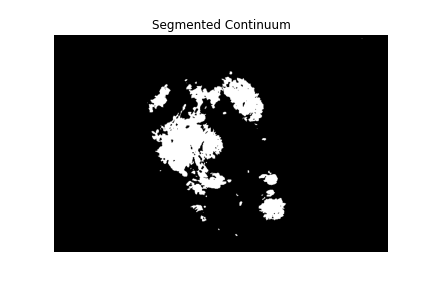
\includegraphics[width=.8\linewidth]{ThesisFilePkg/figures/data/segments.png}
  \caption{After a binary adaptive filter to \ref{fig:binarythreshorig} \cite{scikit}}
  \label{fig:binarythreshafter}
\end{subfigure}
\caption{The result of applying an adaptive binary filter to the original continuum intensity of HARP number 7115}
\label{fig:binarythresh}
\end{figure}
    
    
    \item Second, we group all the pixels that are touching adjacently or diagonally (lines 9 - 20) and filter out groups of pixels that couldn't be considered Penumbras. This is a three-fold process. First, (lines 13-15) we remove groups that are less than 10 pixels in area. The next two filters are only to speed up computation. We then remove all clusters less than 1\% of the size of the largest cluster (lines 16-18) for the same reason we removed small clusters. Finally, of the remaining groups, we keep the largest six clusters (line 20) (at this point, this step usually doesn't filter out many groups unless the AR is noticeably large and fragmented). 
    
    
\begin{figure}[h]
\centering
\begin{subfigure}[b]{.45\textwidth}
  \centering
  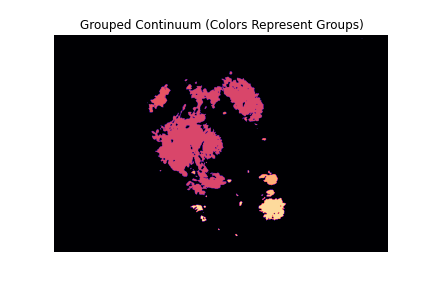
\includegraphics[width=.8\linewidth]{ThesisFilePkg/figures/data/segments_grouped.png}
  \caption{Grouped continuum. Different colors represent different groups}
  \label{fig:grouped}
\end{subfigure}%
\quad
\begin{subfigure}[b]{.45\textwidth}
  \centering
  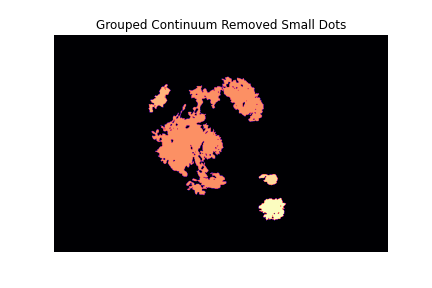
\includegraphics[width=.8\linewidth]{ThesisFilePkg/figures/data/segments_grouped_filtered.png}
  \caption{Grouped continuum after removing small pixel groups and taking the 6 largest from \ref{fig:grouped}}
  \label{fig:groupedfiltered}
\end{subfigure}
\caption{The result of grouping then filtering the AR previously Segmented in figure \ref{fig:binarythresh}. It's important to note that from \ref{fig:grouped} to \ref{fig:groupedfiltered}, the Umbra segment maintains all the filtered pores. That is, we only group regions so we can find Penumbras and we assume Penumbras aren't found in these filtered groups.}
\end{figure}
    
    
    \item Finally, we run through all clusters and determine if they are unimodal (just an Umbra) or bimodal (Penumbra and Umbra). Through experimentation, a value of 21000 is chosen as a benchmark for Umbra / Penumbra difference. That is, if the maximum minus the minimum pixel value was greater than 21000, then the region is bimodal, otherwise, it is unimodal. This number was taken by manually selecting 125 unimodal and bimodal AR images (by eye). If the sub region ($g$) is bimodal, we split it into two subsets with a threshold chosen to be halfway between the maximum and minimum pixel values (line 33). The Penumbra is all the pixels above this value. This Penumbra (as previously mentioned) is subtracted from the Umbra. Otherwise, there is no other work to be done. These segmentation parameters (21000 and halfway between the maximum and minimum) can be adjusted by the user, but sacrifices for computational effectiveness and efficiency had to be made for our specific application of solar flare forecasting.
    
\begin{figure}[h]
\centering
\begin{subfigure}[b]{.45\textwidth}
  \centering
  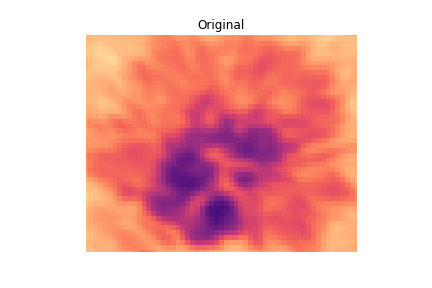
\includegraphics[width=.8\linewidth]{ThesisFilePkg/figures/data/Original_33.0.png}
  \caption{An isolated group of pixels that shows a clear Umbra and Penumbra on the continuum.}
  \label{fig:UmbraPenumbraorig}
\end{subfigure}%
\quad
\begin{subfigure}[b]{.45\textwidth}
  \centering
  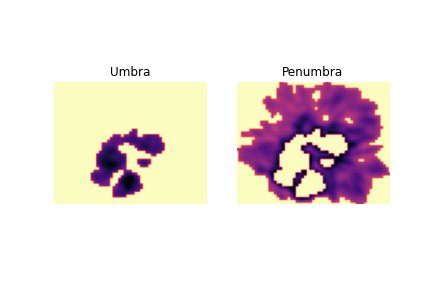
\includegraphics[width=.8\linewidth]{ThesisFilePkg/figures/data/segments_33.0.png}
  \caption{The algorithm recognizes that this subset of the continuum is bimodal, and extracts both the Penumbra and Umbra.}
  \label{fig:UmbraPenumbraseg}
\end{subfigure}
\caption{The algorithm then loops through all of the isolated groups and determines if they are unimodal or bimodal and extracts the Umbra and Penumbra from the image. \ref{fig:UmbraPenumbraorig} shows the original ``recognized" Umbra (this is a subset of the original continuum, which is found in the bottom right corner of the large darkened spot), then \ref{fig:UmbraPenumbraseg} shows the algorithm's determination of Penumbra and Umbra segments. Notice that, as expected, the Penumbra surrounds the Umbra and hugs the edges. Of course, the Umbra in \ref{fig:UmbraPenumbraseg} isn't used, it is only the Penumbra that is eventually subtracted from the Umbra because both sections are included in the original binary mask}
\end{figure}
    
    
\end{enumerate}


\begin{algorithm}
\caption{Umbra and Penumbra Segmentation (\textit{ActiveRegion.assert\_Umbra\_Penumbra()}) }\label{alg:umpum}

\begin{algorithmic}[1]
    \State
    \State \textbf{\textit{/* Step one: Pre-process and threshold the continuum */}}
    \State $C \gets$ Continuum
    \State $C \gets \frac{C - min(C)}{max(C)} \times 255$ \Comment{Bound C by 0 and 255}
    \State $Mask \gets C < localAdaptiveThreshold(C, 5)$ \Comment{Use a square kernel of size 5x5 in the adaptive threshold} 
    \State $Umbra \gets Mask$ \Comment{The Umbra is originally all the pixels from the threshold}
    
    \State
    \State $G \gets groupPixels(Mask)$ \Comment{Group pixels that are adjacent or diagonal}
    
    \State 
    \State \textbf{\textit{/* Step two: Filter invalid groups of pixels */}}
    \For{$g \in G$}
        \If{$size(g) < 10$ pixels}
            \State $G.remove(g)$
        \EndIf
        \If{$size(g) < 0.1 * largest(G)$}
            \State $G.remove(g)$
        \EndIf
    \EndFor
   
    \State $G \gets $ Largest 6 $g \in G$ \Comment{Take only the largest 6 groups (or less)}
    
    \State
    \State \textbf{\textit{/* Step three: For each group $g$, check if it's only Umbra or Penumbra + Umbra */}}
    \State Penumbra $\gets$ Fully false $n \times m$ boolean mask
    \State 
    \For{$g \in G$}
        \State
        \State \textbf{\textit{/* Take the maximum and minimum of the continuum (not bounded) restricted to the subdomain g*/}}
        \State $Max \gets max(Continuum|_g)$ 
        \State $Min \gets min(Continuum|_g)$
        \State 
        \If{$Max - Min > 21000$} \Comment{Umbra and Penumbra}
            \State $t \gets \frac{Max - Min}{2} + Min$
            \State $Penumbra \gets Penumbra \cup ((Continuum > t) \cap g)$
        \EndIf
    \EndFor
    
    \State
    \State $Umbra \gets Umbra \cap \neg Penumbra$
    \State \textbf{Return} $Umbra, Penumbra$ 
\end{algorithmic}
\end{algorithm}


Finally, we are left with two binary masks, the Umbra and Penumbra extracted from the continuum. This is shown in figure \ref{fig:UmbraPenumbrafinal}.


\begin{figure}[h]
    \centering
    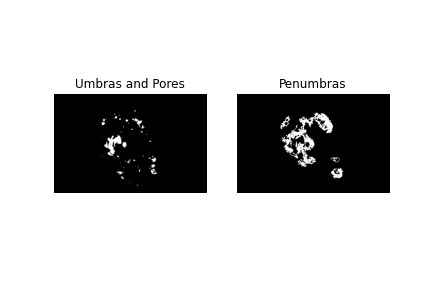
\includegraphics[width=0.7\linewidth]{ThesisFilePkg/figures/data/umbra_penumbra.png}
    \caption{The end product of the segmentation of the Umbra and Penumbra. The left shows the ``Umbra" segment (we call this the Umbra in our feature set, but it really consists of both Umbras and darkened Pores). The left shows the Penumbra segment of the continuum}
    \label{fig:UmbraPenumbrafinal}
\end{figure}

\section{Neutral Line Extraction}

The \textit{Neutral Line} is defined as a continuous subset of an AR such that the line of sight magnetic flux is (theoretically) $0\frac{Mx}{cm^2}$ and the gradient from positive to negative line of sight magnetic flux is relatively high \footnote{In this paper we use a fixed threshold and only include magnetic inversion of the active region where the absolute value of pixels is greater than $150 \frac{Mx}{cm^2}$, a value chosen by Schrijver \cite{schrijver}}. Solar flares occur frequently in these polarity inversion regions with a high magnetic field gradient. \cite{Properties2} show that the length of the neutral line with horizontal shear greater than $80^o$ performed well in a one variable discriminant analysis. This suggests that automatically detecting the neutral lines or regions of high magnetic polarity and polarity inversion could offer more information for solar physics research, flare forecasting methods, and other applications.

The Neutral Line can be extracted in it's own algorithm, which is much simpler and uses a threshold followed by a binary dilation. The algorithm to extract Neutral Lines is shown in \ref{alg:NL}:

First, we lower threshold by the absolute value of the line of sight magnetogram. We use a threshold value of $150 \frac{Mx}{cm^2}$. This leads to two disjoint subsets of the magnetic field showing highly positive and highly negative regions in figure \ref{fig:nlposneg}.


\begin{figure}[h]
    \centering
    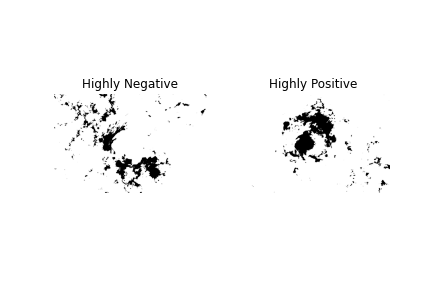
\includegraphics[width=0.5\linewidth]{ThesisFilePkg/figures/data/posneg.png}
    \caption{The result of lower thresholding the original line of sight magnetic field above and below by 150 and -150 $\frac{Mx}{cm^2}$ respectively.}
    \label{fig:nlposneg}
\end{figure}

Clearly, these two subsets are disjoint as a pixel can't be both positive and negative at the same time; but when we dilate the image, the original segments expand slightly (by 5 pixels to be exact, which is an arbitrary number that can be adjusted by the user) shown in figure \ref{fig:nldilated}. This is done in lines 7-8.

\begin{figure}[h]
    \centering
    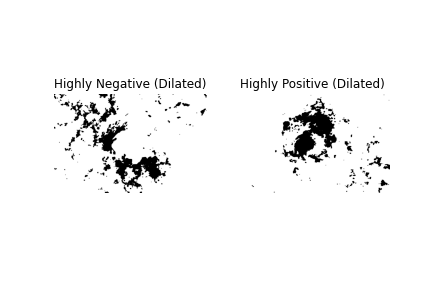
\includegraphics[width=0.5\linewidth]{ThesisFilePkg/figures/data/dilated.png}
    \caption{The result of dilating figure \ref{fig:nlposneg}. Although similar, these subsets are slightly expanded (by 5 pixels)}
    \label{fig:nldilated}
\end{figure}

By taking the intersection of these two binary dilations (line 11), we find strips of magnetic flux that rapidly change from positive to negative. Just like the Umbra and Penumbra algorithm, we group pixels and filter them, then return the union of all groups as the Neutral Line segment (lines 13-27). This is shown graphically in figure \ref{fig:nlfinal}, and is the final Neutral Line segment used in our feature set.


\begin{figure}[h]
    \centering
    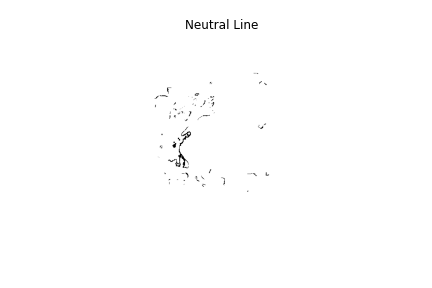
\includegraphics[width=0.7\linewidth]{ThesisFilePkg/figures/data/neutralline.png}
    \caption{The result of intersecting figure \ref{fig:nldilated}, leading to the final Neutral Line.}
    \label{fig:nlfinal}
\end{figure}


\begin{algorithm}
\caption{Neutral Line Segmentation Algorithm (\textit{ActiveRegion.assert\_neutral\_lines(radius ($r$), threshold ($t$))})}\label{alg:nl}
\label{alg:NL}

\begin{algorithmic}[1]

\State
\State \textbf{\textit{/* r is the radius of the kernel used for dilation */}}
\Require $0 < r < min(m,n)$ \Comment{where our image is of size $m\times n$}
\State
\State \textbf{\textit{/* t is the initial threshold value (chosen to be 150 $\frac{Mx}{cm^2}$)}}
\Require $0 < t$

\State
\State \textbf{\textit{/* Bz is the line of sight magnetic field array */}}
\State $mask^{+} \gets$ binaryDilation(Bz $> t$, square($r$)) \Comment{Dilate Positive pixels with an $r \times r$ square kernel}
\State $mask^{-} \gets$ binaryDilation(Bz $< -t$, square($r$)) \Comment{Dilate Negative pixels with an $r \times r$ square kernel}

\State
\State \textbf{\textit{/* The intersection of these two dilations rapidly changes from positive to negative */}}
\State $Mask \gets mask^+ \cap mask^-$ 

\State

\State $G \gets groupPixels(Mask)$ \Comment{Group pixels that are adjacent or diagonal}

\State 
\State \textbf{\textit{/* Step two: Filter invalid groups of pixels */}}
\For{$g \in G$}
    \If{$size(g) < 10$ pixels}
        \State $G.remove(g)$
    \EndIf
    \If{$size(g) < 0.1 * largest(G)$}
        \State $G.remove(g)$
    \EndIf
\EndFor

\State
\State $G \gets $ Largest 6 $g \in G$ \Comment{Take only the largest 6 groups (or less)}
\State
\State \textbf{Return} $\cup_{\forall g \in G}g$ \Comment{The union of all subregions in $G$}
\end{algorithmic}
\end{algorithm}

The final product is a Segmented magnetogram as shown in figure \ref{fig:nlfinal}. 

\section{Background Extraction}

The background is simply the negation of all of the previously defined subgroups.

$$Background \gets \neg(Umbra \cup Penumbra \cup Neutral Line)$$

The background is included to be comprehensive. We do not wish to lose out of any information from the given AR and ignoring everything else other than the Umbra, Penumbra and Neutral Line could cause a loss of information.


\chapter{Judging Criteria}
\label{appendix:judjingcriteria}

It is important to describe how I judged a model, i.e. the metric I will be using to score a model. Most machine learning models operate on the fundamental concept of ``minimizing error". However, this error doesn't have anything to do with the actual practical utility of a model because it may perform better on certain types of datapoints than others. In this study, because my problem is a binary classification one, I am interested in how often my model:

\begin{itemize}
    \item Predicts correctly that a M+ flare will happen in 24 hours (True Positive: TP)
    \item Predicts correctly that a M+ flare will not happen in 24 hours (True Negative: TN)
    \item Predicts incorrectly that a M+ flare will happen in 24 hours (False Positive: FP)
    \item Predicts incorrectly that a M+ flare will not happen in 24 hours (False Negative: FN)
\end{itemize}

\section{TSS Score}
One could imagine that the meaningfulness of each of these categories varies greatly across applications. In one situation, someone could be more interested in TP than TN because a positive has a higher risk factor. In this flare forecasting problem, we are interested primarily in how often we can predict a flare correctly (TP). However, we don't wish to waste valuable resources and assume flares happen more often than they do, so we also wish to minimize FP. For the prior mentioned importance of TP, it is slightly more important to maximize TP than it is to minimize FP, but both are considered in our result. We define the true positive rate ($TPR$) as the \textit{sensitivity} of our model, i.e., the number of correctly predicted positives ($TP$) over the total positives' population (Number of Positives $= TP + FN$):

$$TPR = \frac{TP}{TP + FN}$$

We define the true negative rate ($TNR$) as the \textit{specificity} of our model, i.e., number of correctly predicted negatives ($TN$) over the total negatives' population (Number of Negatives $= TN + FP$):

$$TNR = \frac{TN}{TN + FP}$$

Combining these two scores together, we define Youden's J statistic, referred to in this study as the True Skill Statistic ($TSS$), as:

$$TSS = TPR + TNR - 1$$

as a number that spans limits below at $-1$ when every positive was called a negative and every negative was labeled a positive - A perfectly negative score \footnote{Often in literature, $TSS \geq 0$ because we can adapt the predicted label to the observed label, treat 0's as 1's and 1's as 0's}. $TSS$ equals $0$ when every datapoint is labeled positive / negative (this property combats accuracy inflation in an unbalanced feature set) and $1$ when every positive was labeled a positive and every negative was labeled a negative - A perfect Model. In this study, and the analysis of feature sets against each other, I use the $TSS$ score as my primary metric, but there are two more important metrics that I continually use to highlight certain characteristics of models: the $f1$ score and the Heidke Skill Score $HSS$. I also include accuracy as a simple, understandable metric.


\section{F1 Score}
Rather than combining the true positive rate and true negative rate, the $f1$ score relies on the combination of precision and recall. Precision shows how much \text{we can trust} a model when it gives a positive prediction (probability of a positive conditioned on being labeled positive). Precision is equal to the correct predicted positives over the predicted positives:

$$Precision = \frac{TP}{TP + FP}$$

Recall (same as TPR) measures model \textit{sensitivity}. It shows how much we can trust the model \text{in order to predict} a flare will happen (probability of a positive conditioned on being actually positive). Recall is equal to the correct predicted positives over the observed positives:

$$Recall = TPR = \frac{TP}{TP + FN}$$

The $f1$ score is simply the (sometimes weighted) harmonic mean of these two metrics:

$$f1 = \frac{2}{\frac{1}{Precision} + \frac{1}{Recall}}$$

The harmonic mean is chosen to punish extreme values. Both precision and recall have $TP$ in the numerator so it makes more sense to average their denominators of unequal values, hence the use of the harmonic mean.

The problem with the $f1$ score comes with imbalanced feature sets. In practice, there is approximately a near 1:100 \footnote{Within 24 hours, the ratio explained later in this section is for HARP numbers and not individual data points} ratio of flaring : non flaring ARs. Therefore, $FP$ will be artificially deflated because our model will learn that there are fewer positives than negatives. Therefore, the precision will appear very high. 

\section{Heidke Skill Score}
The Heidke Skill Score ($HSS$), known as the Kappa Score outside of climatology, is slightly more complex and shows the improvement over any type of standard forecast accuracy (which we have chosen to be the chance accuracy ($E$)). The accuracy (percent correct) of a model is equal to $\frac{TP + TN}{N} = \frac{TP + TN}{TP + TN + FP + FN}$. The perfect value for accuracy is 1. Accuracy is maximized when all data points ($x$) that are observed to be positive ($x = 1$) are correctly labeled ($\hat{x}$) as positive ($\hat{x} = 1$). The same for negative points. The reference accuracy ($E$) is equal to the probability that our model correctly guessed a label merely by random chance:

$$E = p(x = 1 \quad and \quad \hat{x} = 1) \quad or \quad p(x = 0 \quad and \quad \hat{x} = 0)$$
$$= p(x = 1)p(\hat{x} = 1) + p(x = 0)p(\hat{x} = 0)$$
$$ = p(x = 1)(\frac{TP + FP}{N}) + p(x = 0)(\frac{FN + TN}{N})$$

Where $N = TP + TN + FP + FN$ and $p(x)$ is fixed (across all possible models) as the probability of each classification in the given abstracted space. These are fixed constants that I will derive in the next section. The $HSS$ score is the ratio of the observed performance (accuracy) minus the probability that a datapoint is correctly classified ($E$) over the perfect performance ($1$) minus the probability that a datapoint is correctly classified ($E$):

$$HSS = \frac{Model Accuracy - E}{Perfect Accuracy - E}$$

Note that often $HSS$ is simplified to the expression below:

$$HSS = \frac{2((TP)(TN)-(FP)(FN))}{(TP + FP)(FP + TN) + (TP + FN)(FN + TN)}$$

This simplification comes from defining $p(x = 1) = \frac{TP + FN}{N}$ and $p(x = 0) = \frac{TN + FP}{N}$. However, in this study, I have access to years of flaring data and $p(x)$ can be estimated by the frequency of flares in the past, which I will describe further in the next section.

These three metrics: $TSS$, $f1$ and $HSS$ will be used in my results section to discuss how a certain model performed on an individual feature set, but the $TSS$ score will be used to rank models because I believe it is most fit by fixing the imbalanced feature set problem. Looking at the raw $TP$, $TN$, $FN$, $FP$ rates alone is also useful because it shows each model's strength's and weaknesses. Does a model tend to perform really well at finding flares? Can we trust the model when it makes a positive / negative response? These are all important considerations for each model we use to generate a solar flare forecast that I will analyse in my findings section.


\chapter{False Rates for the Full and Segmeted feature sets}
\label{appendix:fprfnrother}

\begin{figure}[h]
\centering
\begin{subfigure}[b]{.45\textwidth}
    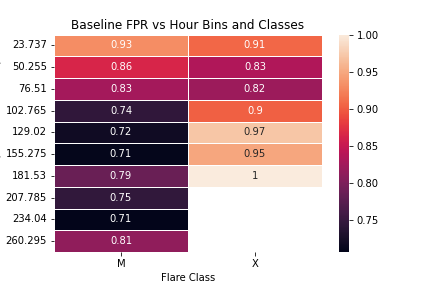
\includegraphics[width=\linewidth]{ThesisFilePkg/figures/findings/baselineFPR.png}
\end{subfigure}
\begin{subfigure}[b]{.45\textwidth}
    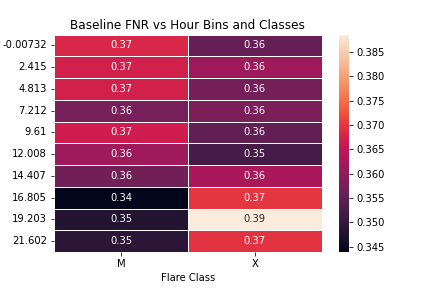
\includegraphics[width=\linewidth]{ThesisFilePkg/figures/findings/baselineFNR.png}
\end{subfigure}
\label{fig:basfr}
\caption{The false negative and positive rates for the Full feature set. Unlike the Segmented feature set, X flares are predicted correctly less frequently than the M flares.}
\end{figure}


\begin{figure}[h]
\centering
\begin{subfigure}[b]{.45\textwidth}
    \includegraphics[width=\linewidth]{ThesisFilePkg/figures/findings/SHARPsFPR.png}
\end{subfigure}
\begin{subfigure}[b]{.45\textwidth}
    \includegraphics[width=\linewidth]{ThesisFilePkg/figures/findings/SHARPsFNR.png}
\end{subfigure}
\label{fig:shpfr}
\caption{The false negative and positive rates for the SHARPs feature set. Unlike the Segmented feature set, X flares are predicted correctly less frequently than the M flares.}
\end{figure}

\end{document}